
\documentclass[12pt,a4paper]{scrartcl}

% scrartcl ist eine abgeleitete Artikel-Klasse im Koma-Skript
% zur Kontrolle des Umbruchs Klassenoption draft verwenden


\usepackage[utf8]{inputenc}
% \usepackage[latin1]{inputenc} %  Alternativ unter Windows
\usepackage[T1]{fontenc}
\usepackage[ngerman]{babel}
\usepackage{url}

\usepackage[pdftex]{graphicx}
\usepackage{latexsym}
\usepackage{amsmath,amssymb,amsthm}
\usepackage{mathtools}
\usepackage{ae,aecompl}
\usepackage{blindtext}
\setcounter{secnumdepth}{5}
%\usepackage{graphicx}
\graphicspath{ {./images/} }
\usepackage{hyperref}
\usepackage{acronym}
\usepackage{subcaption}
\usepackage[dvipsnames]{xcolor}
\usepackage{tikz}
\usepackage{tkz-euclide}
\usepackage{pgfplots}
\usetikzlibrary{matrix, positioning}

\usepackage[linesnumbered,lined,boxed,commentsnumbered]{algorithm2e}

%\usepackage[demo]{graphicx}
\usetikzlibrary{arrows,automata, matrix,chains,positioning,decorations.pathreplacing,arrows}

% Abstand obere Blattkante zur Kopfzeile ist 2.54cm - 15mm
\setlength{\topmargin}{-15mm}


\numberwithin{equation}{section} 

% einige Abkuerzungen
\newcommand{\C}{\mathbb{C}} % komplexe
\newcommand{\K}{\mathbb{K}} % komplexe
\newcommand{\R}{\mathbb{R}} % reelle
\newcommand{\Q}{\mathbb{Q}} % rationale
\newcommand{\Z}{\mathbb{Z}} % ganze
\newcommand{\N}{\mathbb{N}} % natuerliche
\def\Arrow{\raisebox{3\height}{\scalebox{1}{$\xRightarrow[.]{.}$}}}
\newcommand*{\putunder}[2]{	{\mathop{#1}_{\textstyle #2}}}


\makeatletter
\renewcommand\paragraph{\@startsection{paragraph}{4}{\z@}%
	{-2.5ex\@plus -1ex \@minus -.25ex}%
	{1.25ex \@plus .25ex}%
	{\normalfont\normalsize\bfseries}}
\makeatother
\setcounter{secnumdepth}{4} % how many sectioning levels to assign numbers to
\setcounter{tocdepth}{4}    % how many sectioning levels to show in ToC

\begin{document}
  % Keine Seitenzahlen im Vorspann
  \pagestyle{empty}

  % Titelblatt der Arbeit
  \begin{titlepage}

    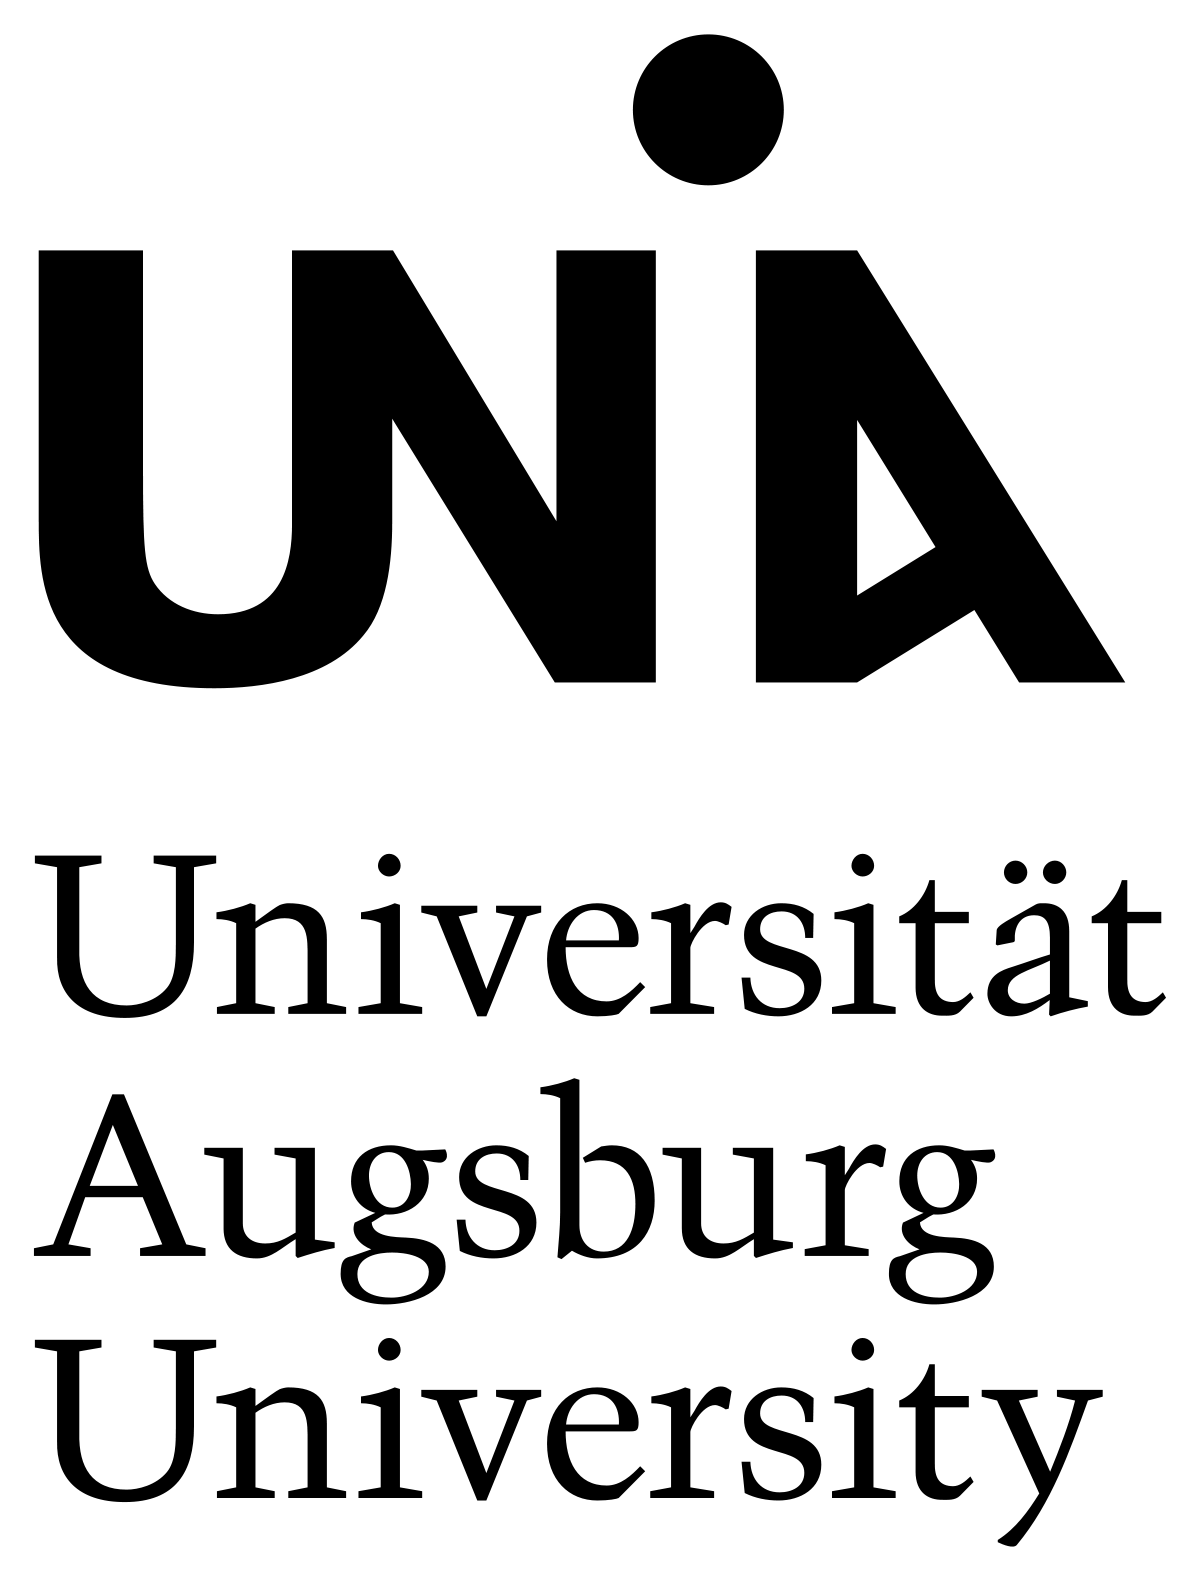
\includegraphics[scale=0.05]{logo_uni} 
    \vspace*{2cm} 

 \begin{center} \large 
    
    Bachelorarbeit
    \vspace*{2cm}

    {\huge Titel der Bachelorarbeit: Image Analysis for Food Safety and Health}
    \vspace*{2.5cm}

    Name des Autors: TEMKENG Thibaut
    \vspace*{1.5cm}

    Datum der Abgabe: Ende Oktober
    \vspace*{4.5cm}


    Betreuung: Name der Betreuer/ des Betreuers:Shou Liu \\[1cm]
    Fakultät für Embedded Intelligence for Health Care and Wellbeing \\[1cm]

  \end{center}
\end{titlepage}




    \section*{Erklärung}
  
  Ich  versichere  wahrheitsgemäß,  die  Arbeit selbstständig verfasst,  alle  benutzten  Hilfsmittel  vollständig  und  genau  angegeben  und  alles kenntlich  gemacht  zu  haben,  was  aus  Arbeiten  anderer  unverändert  oder  mit  Abänderungen entnommen  wurde,  sowie die Satzung  der  Universität Augsburg  zur  Sicherung guter wissenschaftlicher Praxis in der jeweils gültigen Fassung beachtet zu haben.
  \\[2ex] 
  
  \noindent
  Ort, den Datum\\[5ex]
 

\newpage
   % Inhaltsverzeichnis
 \tableofcontents
%\newpage
%\listofalgorithmes


  % Ab sofort Seitenzahlen in der Kopfzeile anzeigen
  \pagestyle{headings}
 \newpage
%
%\section{Abkürzungsverzeichnis}
\begin{acronym}[THIBAUT]
	\acro{KNN}{Künstliches neuronales Netz}
	\acro{CNN}{Convolutional Neural Network}
	\acro{KI}{Künstliche Intelligenz}
	\acro{NN}{neuronales Netz}
	\acro{ConvL}{Convolutional Layer}
	\acro{FCL}{Fully Connected Layer}
	\acro{PooL}{Pooling Layer}
	\acro{ILSVRC }{ Large Scale Visual Recognition Challenge}
	\acro{DNN}{Tiefe neuronale Netze}
	\acro{ML}{Maschine Lernen}
	\acro{DSC}{Depthwise Separable Convolution}
\end{acronym}
\newpage
\section{Einleitung}



%%%%%%%%%%%%%%%%%%%%%%%%%%%%%%%%%
 \newpage  % neuer Abschnitt auf neue Seite, kann auch entfallen
%%%%%%%%%%%%%%%%%%%%%%%%%%%%%%%%%
 
\section{Grundlagen}\label{Grundlagen}
Im folgenden Kapitel werden die Grundlagen von neuronalen Netzwerken beschrieben, beginnend mit künstlichen neuronalen Netzen, gefolgt von einem Abschnitt über Faltungsneuronale Netzwerke und
zum Abschluss ein Abschnitt über die verwendeten Datensätze und Bibliotheken.
\subsection{Künstliche neuronale Netze}
\subsubsection{Neuron}
Ein künstliches Neuron\cite{kneuron} ist eine mathematische Funktion, die das Verhalten vom biologischen Neuron nachbildet. Künstliche Neuronen sind elementare Einheiten in einem \ac{KNN}. Das künstliche Neuron empfängt einen oder mehrere Inputs und bildet sie auf einen Output ab. Normalerweise wird jeder Eingabe $ x_i $ separat mit einem Gewicht $ w_i $ multipliziert und danach aufsummiert und zum Schluss wird die Summe durch eine Funktion geleitet, die als Aktivierungs- oder Übertragungsfunktion bekannt ist.Eine schematische Darstellung eines künstlichen Neurons ist in Abbildung \ref{fig:Fneuron}
zu sehen.

\begin{figure}[h]
	\centering
	\begin{tikzpicture}[
	init/.style={
		draw,
		rectangle, rounded corners,
		font=\Large,
		inner sep=2pt,
		join = by -latex
	},
	squa/.style={
		draw,
		inner sep=2pt,
		font=\Large,
		join = by -latex
	},
	start chain=2,node distance=13mm
	]
	\node[on chain=2] 
	(x2) {\textbf{$x_j$}};
	\node[on chain=2,join=by o-latex] 
	{\textbf{$w_j$}};
	\node[on chain=2,init] (sigma) 
	{$z= \sum_{i =1}^{n}{x_iw_i +b} $};
	\node[on chain=2,squa,label=above:{\parbox{2cm}{\centering Aktivierungs\\funktion $ f $}}]   
	{$f(z)$};
	\node[on chain=2,label=above:Output,join=by -latex] 
	{$y$};
	\begin{scope}[start chain=1]
	\node[on chain=1] at (0,1.5cm) 
	(x1) {\textbf{$x_1$}};
	\node[on chain=1,join=by o-latex] 
	(w1) {$w_1$};
	\end{scope}
	\begin{scope}[start chain=3]
	\node[on chain=3] at (0,-1.5cm) 
	(x3) {$x_n$};
	\node[on chain=3,label=below:Gewichte,join=by o-latex] 
	(w3) {$w_n$};
	\end{scope}
	\begin{scope}[start chain=4]
	\node[on chain=4] at (0,-.75cm) 
	(x4) {\vdots};
	\node[on chain=4,join=by o-latex] 
	(w4) {\vdots};
	\end{scope}
	
	\begin{scope}[start chain=5]
	\node[on chain=5] at (0,.75cm) 
	(x5) {\vdots};
	\node[on chain=5,join=by o-latex] 
	(w5) {\vdots};
	\end{scope}
	\node[label=above:{\parbox{2cm}{\centering Bias\\b }}]  (b)[above =0.7cm and 4cm of sigma] {};
	
	\draw[-latex] (w1) -- (sigma);
	\draw[-latex] (w3) -- (sigma);
	\draw[-latex] (w4) -- (sigma);
	\draw[-latex] (w5) -- (sigma);
	\draw[o-latex] (b) -- (sigma);
	
	\draw[decorate,decoration={brace,mirror}] (x1.north west) -- node[left=10pt] {Inputs} (x3.south west);
	\end{tikzpicture}
	\caption{Funktionsweise eines künstlichen Neurons }
	\label{fig:Fneuron}
\end{figure}


Künstliche Neurone können aufgestapelt werden, um eine Schicht(\textit{Layer}) zu bilden.Ein \ac{KNN} besteht aus einer oder mehreren Schichten und je nach seiner Position in einem \ac{NN} wird eine Schicht anders genannt: Eingangsschicht(\textit{Input Layer}) bzw. Ausgabeschicht(\textit{Output Layer}), wenn das Layer die Eingangsdaten bzw. Ausgabedaten des neuronalen Netzes darstellt und versteckte Schicht(\textit{Hidden Layer}), wenn es keine Eingang- oder Ausgabeschicht ist.Ein kurzer Überblick über die Darstellung von \acsp{KNN} kann sich in Abbildung \ref{KNN} verschafft werden.

\subsubsection{Merkmalskarten(Feature-Maps)}
Die Ausgabe einer Schicht wird als Aktivierungskarten oder Feature-Map(s) bezeichnet. Die Anzahl von Feature-Maps in einer Schicht ist gleich die Anzahl der Ausgabekanäle(\textit{output channels}) bzw: Tiefe(\textit{depth}) dieser Schicht.
In einer Faltungsschicht ist ein Feature-Map immer zweidimensional, während die Dimension eines Feature-Maps in einem \ac{FCL} nur von der des Inputs abhängt, genauer gesagt,für ein n-dimensionales Inputs ist ein Feature-Map $ (n-1) $dimensional.
Wie die Feature-Maps berechnet werden, hängt sehr vom Schichttyp ab. Es wird beispielsweise in einer Faltungsschicht die Faltungsoperation mehrmals auf die Eingabe angewendet und jedes Mal wird ein neues Feature-Map erhalten.

\subsubsection{Filters}\label{Filter}
Ein Filter ist eine kleine Matrix, die die Extraktion von Features ermöglicht.
Die modernen Architekturen von \ac{CNN} verwendet immer mehr Filter (mindestens $ 2000 $), um bessere Ergebnisse zu erzielen. Wegen der zufällige Initialisierung von Filtern und ihrer großen Anzahl im \ac{CNN} kann es vorkommen, dass mehrere Filter das gleiche Feature extrahieren, solche Filter werden als Redundant bezeichnet, oder dass Filter genau das Gegenteil von dem filtern, was wir wollen, nämlich unwichtige Informationen, deshalb werden während des Trainings die Filterparameter ständig geändert. Zwei nichtlineare Filter, d. h. Filter, die nicht proportional zueinander sind, lernen unterschiedliche Dinge.Man kann also daraus schließen, dass je größer die Anzahl an Filter ist, desto mehr Features gefiltert werden können oder besser sind die Ergebnisse, aber das ist in Allgemein falsch, da die guten Ergebnisse sehr stark davon abhängen, wie die Filter im CNN aufgestapelt sind. Zu viele Filtern in einem \ac{CNN} können dazu führen, dass das \ac{CNN} sowohl gute Features als auch schlechte schneller lernt und zu wenige Filter schränken die Kapazität des \ac{CNN} ein,  wichtige Features zu extrahieren, denn irgendwann wird es vorkommen, dass jedes Filter etwas Wichtiges gelernt hat, aber noch mehr Informationen werden benötigt, um die Trainingsdaten zu erklären.
Es ist also wichtig die richtige Anzahl von Filtern zu finden.


\begin{itemize}
	%- formalisierte Entsprechung der Nervenzelle besteht aus\\
	
	%	\item \textbf{Aktivierungszustand} (\textit{Activation state}) Er gibt oder definiert den aktuellen Zustand eines Neurons.
	%	\item \textbf{Propagierungsfunktion} (\textit{propagation function}) Sie bestimmt den gesamten Input(auch Netto-Input) des Neurons.\textcolor{red}{Sie legt fest, wie die Eingabe des Neuron aufzuarbeiten ist} Die häufigste verwendete Propagierungsfunktion ist die summe der gewichteten Eingaben, die das Neuron von anderen Neuronen erhält.
	%	\item \textbf{Aktivierungsfunktion} ( \textit{activation function}) Sie legt fest, wie der nächste Aktivierungszustand des Neurons aus dem Netto-Input und dem aktuellen Aktivierungszustand berechnet wird. Es gibt  zahlreiche Aktivierungsfunktionen(zB. ELU, LeakyReLU, Sigmoid, Softmax, Maxout, tanh), die auch unterschiedliche Einflüsse auf die Ausgabe eines Neurons. Die verbreitetsten Aktivierungsfunktionen sind die Logistische(Sigmoid, Gleichung \ref{Sigmoid}, Graph \ref{fig:sigmoid}), \textbf{Re}ctified \textbf{l}inear \textbf{u}nit(ReLU, Gleichung \ref{Relu}, Graph\ref{fig:relu},) Relu und Softmax(Gleichung \ref{Sotfmax})  Funktion. 
	%	
	%		\begin{equation}
	%	\label{Relu}
	%	ReLU = max(x, 0)
	%	\end{equation}
	%	
	%	\begin{equation}
	%	\label{Sigmoid}
	%	Sigmoid(x) =  \frac{\mathrm{e^x} }{\mathrm{e^x +1} }
	%	\end{equation}
	%	
	%	\begin{equation}
	%	\label{Sotfmax}
	%	Softmax(x_1, x_2, \cdots, x_n) = \frac{(e^{x_1}, ê^{x_2}, \cdots, e^{x_n})}{\sum_{i =1}^{n}{e^{x_i}}}
	%	\end{equation}
	%	
	%	
	%	Nach \cite{9} sollten die Aktivierungsfunktionen vorgezogen werden, die mehr von folgenden Eigenschaften aufweisen:	
	%	
	%	\textbf{Nichtlinearität:} Bei einem mehrschichtigen Netz ist es nicht sinnvoll eine lineare Aktivierungsfunktion zu benutzen, denn ein solches Netz in ein einschichtiges Netz immer überführt werden kann und es ist bekannt, dass ein mehrschichtiges Netz mehr als ein einschichtiges Netz leisten kann.
	%
	%	\textbf{Überall differenzierbar:} Diese Eigenschaft ermöglicht, gradientenbasierende Optimierungsverfahren zu verwenden.
	%	
	%	\textbf{Wertebereich:} Die gradientenbasierende Lernmethode ist stabiler, wenn der Wertebereich der Aktivierungsfunktion endlich ist und wenn es dagegen unendlich ist, ist das Lernen im Allgemeinen effektiver.
	%	
	%	\textbf{Monotonie:} Wenn die Aktivierungsfunktion monoton ist, so ist die Fehleroberfläche eines einschichtigen Netz immer konvex,\textcolor{red}{was bedeutet, dass es nur ein optimales Minimum gibt und das Optimierungsverfahren immer besser wird}.
	%	
	%	\textbf{Identität in 0} ( $ {\displaystyle f(x)\approx x} $ wenn  $ {\displaystyle x\approx 0} $): Diese Eigenschaft ermöglicht einen schnellen Training, wenn die Gewichte zufällig initialisiert sind und wenn die Aktivierungsfunktion in der Nähe von Null nicht gegen die Identität konvergiert, muss bei der Initialisierung der Gewichte besonders sorgfältig vorgegangen werden.
	%	
	%	
	%	\textbf{ Sigmoid-Aktivierungsfunktion} Obwohl die Sigmoid-Funktion leicht anwendbar und differenzierbar ist, wird sie nach und nach auch nicht mehr verwendet, denn sie zum Beispiel das Problem des verschwindenden Gradienten(\textit{vanishing gradient problem}) nicht löst, was die Leistung tiefer neuronaler Netze stark beeinträchtigt und sie konvergiert sehr langsam.
	\item  
\end{itemize}

\subsubsection{Entwicklung von Künstlichen Neuronalen Netzen } \label{Entwicklung}

%\textbf{\ac{CNN} Vorteile ca va plutôt en haut}\\ 
%Die Verwendung von \acsp{ConvL} ermöglicht die Erkennung und die Entnahme relevanter Merkmale aus den Netzeingangsdaten, was eine Vorverarbeitung der Netzeingangsdaten vermeidet. \acsp{ConvL} machen \acsp{CNN} robuster, denn obwohl es Rauschen in den Eingangsdaten gibt, schafft es immer noch die relevanten Informationen zu extrahieren.Zusätzlich sind \ac{ConvL}  gegenüber Veränderungen, die den Inhalt der Daten nicht ändern, unempfindlich, also wird ein Bild immer gleich klassifiziert werden, obwohl es z.B rotiert oder ein Bisschen verschoben ist.Ein anderer Hauptvorteil von \ac{ConvL} ist die deutliche Reduzierung der Speicheranforderung im Vergleich mit \acsp{FCL} 
%\\textbf{künstliches Neuron}.\\


\subsection{Convolutional Neural Network}
\subsubsection{Feedforward }
%\paragraph{Layer in \ac{CNN}}
\paragraph{Input Layer}\label{InputLayer}
Die Eingangsschicht stellt die Eingangsdaten dar. Hier müssen die Eingangsdaten dreidimensional sein.Also die Eingangsdaten von \ac{CNN}  haben immer die folgende Form $ W\times H\times D $ wobei $ (W, H) $ der räumlichen Dimension und $ D $ die Tiefe der Daten entspricht. Z.B  $ 100\times100 \times3 $ für ein RGB-Bild und $ 224\times224\times1 $ für ein Graustufenbild.


\paragraph{Faltungsschicht}\label{ConvL}
Die wichtigste Sicht bzw. der Hauptschicht in einem \ac{CNN} ist die Faltungsschicht(\emph{Convolution Layer}).
Die Eingabedaten eines \ac{CNN} besteht auf jedenfalls aus wichtigen und unwichtigen Informationen.Als wichtige und unwichtige Informationen haben wir z.B die starke Präsenz der weißen Farbe in einer Muschelsuppe bzw. die Präsenz eines Menschen, wenn man verschieden Ernährungsklasse klassifizieren möchte. Während des Trainings eines \ac{CNN} wird versucht, diese relevanten Informationen aus den Daten zu entnehmen und die irrelevanten auszuschließen. Alles was ein \ac{CNN} aus den Eingabedaten nutzt, um die Daten zu bestimmter Klassen zuzuordnen, wird als Feature bezeichnet.
Das einzige bzw. das Hauptziel einer Faltungsschicht besteht darin, die Features aus seinen Inputdaten herauszuziehen.
Dass eine Faltungsschicht in der Lage ist, Features selbst zu extrahieren, ohne dass man sie hinweist, was wichtig ist und was nicht, ist wirklich beeindruckend,Aber die Art und Weise, wie sie es tut, ist noch beeindruckender.

In einem \ac{ConvL} wird die sogenannte Faltungsoperation(\emph{convolution operation}) durchgeführt,dabei wird das komponentenweises Produkt(\textit{Hadamard-Product}) zwischen einem kleinen Bereich der Eingabedaten und einem Kernel durchgeführt und dann die ganze aufsummiert. Eine Illustration der Faltungsoperation ist in der Abbildung \ref{fig:Faltungsoperation1} zu sehen. Die Resultante der Faltungsoperation wird die Aktivierung des Neurons genannt.Sollte diese Aktivierung des Neurons null sein, dann sagt man, dass das Neuron "\textit{nicht aktiv}"{} ist und sonst ist es \textit{aktiv}.Die null Aktivierung bedeutet, dass das vom Filter gesuchte Feature nicht gefunden wurde. Je stärker oder größer die Aktivierung eines Neurons ist, desto höher ist die Wahrscheinlichkeit, dass das vom Filter gesuchte Feature gefunden ist(siehe Abbildung \ref{fig:Faltungsoperation2}).
Um diese Faltungsoperation durchzuführen, muss einige Hyperparameter vordefiniert sein, und zwar:

\begin{itemize}
	\item \textbf{Anzahl und Größe von Filtern}\\
	Die Anzahl an Filters gibt nicht nur an, wie viele Filter in dem \ac{ConvL} verwendet werden, sondern auch ,wie oft die Faltungsoperation auf die Eingabe durchgeführt wird, d.h die Anzahl der Feature-Maps oder die Tiefe der Schicht.
	Anstatt das ganze Bild zu betrachten, wenn man auf der Suche nach einem Feature ist, was mit der Tatsache gleichbedeutend ist, dass jedes Neuron der Schicht mit allen Neuronen der vorherigen verbunden ist, wird nur einen lokalen Bereich des Bildes betrachtet, wir verbinden also jedes Neuron nur mit einem lokalen Bereich der Bild. Dieser lokaler Bereich wird als Empfangsfeld(\emph{receptive field}) des Neurons bezeichnet und entspricht der Filtergröße.Es ist zu beachten, dass die Filtergröße nur der räumlichen Dimension des Filters entspricht. Die Tiefe des Filters ist gleich die vom Input, also für ein $ (100, 100, 3) $ Bild haben alle Filter die Tiefe $ 3 $.	
	Die Verwendung von solchen kleinen Filtern ist die Hauptidee hinter einer Faltungschicht. Filter haben im Allgemein eine kleine räumliche Dimension wie z.B $ 2\times 2 $, $3 \times3 $  oder  $5 \times 5$, sonst verliert man einen großen Vorteil von \ac{ConvL}, der darin besteht, die Speicheranforderung deutlich zu reduzieren, indem es die Gewichte verteilt. 
	
	\begin{figure}[h]
		\centering
		\caption{Einfluss der Schrittgröße auf die Größe der Feature-Maps}
		\begin{subfigure}{.5\textwidth}
			\centering
			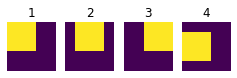
\includegraphics{stride1}
			\caption{\emph{Schrittgröße=(1,1) } }
			\label{fig:stride1}
		\end{subfigure}%
		\begin{subfigure}{.5\textwidth}
			\centering
			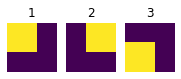
\includegraphics{stride2}
			\caption{ \emph{Schrittgröße=(2,2) } }
			\label{fig:stride2}
		\end{subfigure}
	\end{figure}
	\item  \textbf{Schrittgröße}(\emph{Stride})\\
	
	Da ein Filter nur einen kleinen Bereich des Bilds wahrnehmen kann,wird eine Schrittgröße verwendet, um die Bewegung des Filters auf dem Bild zu steuern.Das Filter wird über das Bild von links nach rechts, von oben nach unten bewegt. Sei $ S:=(n,m) $  die Schrittgröße, dann wird das Filter von $ n $ Pixeln nach rechts für jede horizontale Bewegung des Filters und $ m $ Pixeln nach unten für jede vertikale Bewegung des Filters bewegt(siehe Abbildung \ref{fig:stride1} und \ref{fig:stride2}).Wie die folgende Tabelle zeigt,hängt die räumliche Dimension des Outputs sehr von der Schrittgröße ab.
	
	\begin{table}[h]
		\centering
		\begin{tabular}{|c|c|c|c|c|}
			\hline
			\textbf{Imagegröße} & \textbf{\emph{Stride}} & \textbf{\emph{Filtergröße}} & \textbf{\textit{Output (räumliche Dim.)}}&\textbf{\emph{Mit Padding}}\\ \hline
			$ (100, 100, 3) $ &{$ (1,1) $ }& $ (1,1) $ &{$ (100,100) $ }&$ (100,100) $ \\ \hline
			$ (100, 100, 3) $ &\textcolor{red}{$ (1,1) $ }& $ (3,3) $ &\textcolor{red}{$ (98,98) $ }&$ (100,100) $ \\ \hline
			$ (100, 100, 3) $ &\textcolor{red}{$ (2, 2) $ } & $ (3,3) $ &\textcolor{red}{$ (49,49) $ }&$ (50,50) $ \\ \hline
			$ (100, 100, 3) $ &$ (1,1) $ & \textcolor{blue}{$ (4,4) $ }&\textcolor{blue}{$ (97, 97) $ } & $ (100, 100) $\\ \hline
			$ (100, 100, 3) $ &$ (1,1) $ & \textcolor{blue}{$ (10,10) $ }&\textcolor{blue}{$ (91, 91) $ } &$ (100, 100) $\\ \hline
		\end{tabular}
		\caption{Auswirkung von Schrittgröße,Filtergröße und Padding auf Output eines $ (100, 100, 3) $ Bild.}
		\label{tab:Stride and filter size}
	\end{table}
	
	\item \textbf{\textit{Padding}}\\
	Mit einem großen Filter lernt man in der Regel "mehr"{} als mit einem kleinen.Aber wie es in der Tabelle \ref{tab:Stride and filter size} zu sehen ist, habe man eine Reduktion der Dimension, wenn ein Filter mit Filtergröße $ >1 $ angewendet wird und um die Dimension zu behalten, wird vor der Anwendung der Filter auf das Bild eine Füllung(\textit{padding}) an den Rändern des Bilds gemacht. Diese Füllung ermöglicht erstens den Entwurf immer tiefer Netzwerke, denn es gibt nach jedem \ac{ConvL} einen kleinen Dimensionverlust und zweitens,dass die Information an Rändern nicht zu schnell verschwunden werden.Um die Ränder einer Eingabe zu füllen, werden sehr oft Nullen (\textit{zero padding}) verwendet, oder die Pixel, die an der Grenze liegen, werden wiederholt.
	
\end{itemize}
In einem \ac{CNN} mit mehreren \acsp{ConvL} beschäftigen sich die ersten \acsp{ConvL} mit dem Erlernen einfacher Merkmale wie Winkel, Kanten oder Linien und je tiefer das \ac{CNN} ist, desto komplexer sind die extrahierten Merkmale. Das liegt daran, dass jede nachfolgende Schicht einen größeren Bereich des Originalbildes betrachten oder \glqq sehen \grqq{} kann.Nehmen wir an,dass die zwei ersten Layers eines \acsp{CNN} Filter von Größe $ 3\times 3 $  und ein \textit{Stride} $ =(1,1) $ verwenden.Die erste Schicht betrachte immer $ 3\times3 $ benachbarte Pixel des Originalbildes und speichert seine Aktivierung auf einem Pixel. Jetzt wenn die zweite \ac{ConvL}  $ 3\times3 $ benachbarte Pixel betrachtet, betrachtet sie eigentlich  $ 5\times5 $ benachbarte Pixel des Originalbildes.Wir können uns deshalb vorstellen, dass irgendwo in späteren Schichten Filter das gesamte Originalbild betrachten.
% 
% also die früher entdeckten Features werden kombiniert, um komplexe Features wie einen Kreis zu bilden .Eine Vorverarbeitung der Netzeingangsdaten zur Extraktion der relevanten Information nicht mehr nötig. 
\begin{figure}[h]
	\centering
	\begin{subfigure}{\textwidth}
		\centering
		\caption{Matrixdarstellung}
		\newbox\dumbox
		\newcommand{\mymark}[2]{%
			\setbox\dumbox=\hbox{#2}%
			\hbox to \wd\dumbox{\hss%
				\tikz[overlay,remember picture,baseline=(#1.base)]{ \node (#1) {\box\dumbox}; }%
				\hss}%
		}
	
		
		
		\[ \putunder{\begin{array}{|*{9}{c}|}
			\hline
			\mymark{t}{0}& 0& 3&  3& 3& 0&  \mymark{s}{0}& 0& 0\\ 
			0& \mymark{f}{2}& 0&  3& 2& 0&  0& 2& 0\\ 
			2& 0& \mymark{t1}{2}&  2& 0& 2&  2& 0& \mymark{s1}{2}\\ 						
			\mymark{q}{1}& 1& 1&  \mymark{r}{1}& 1& 1&  1& 1& 1\\ 			
			1& 0& 1&  0& 2& 0&  1& 0& 1\\ 
			0& 0& \mymark{q1}{1}&  2& 0& \mymark{r1}{2}&  0& 0& 1\\ 						
			\mymark{b}{1}& 1& 1&  1& 1& 1&  \mymark{j}{1}& 3& 1\\ 
			3& 0& 3&  1& 2& 0&  3& \mymark{f1}{0}& 3\\ 
			0& 3& \mymark{b1}{0}&  2& 0& 2&  0& 0& \mymark{j1}{0}\\  \hline
			\end{array} }{\text{(9,9)Bild}}  
		\quad \quad \times  \quad \quad
		\putunder{\begin{array}{*{3}{|c}|}
			\hline
			0&0&0 \\ \hline
			0&1&0 \\ \hline
			1&0&1\\ \hline
			\end{array}}{Filter}  
		\quad \quad = \quad \quad
		\putunder{ \begin{array}{ *{3}{|c}|}
			\hline
			\mymark{v}{6}&6&\mymark{ss}{6} \\ \hline
			\mymark{qq}{1}&\mymark{rr}{6}&1 \\ \hline
			\mymark{bb}{0}&6&\mymark{jj}{0}\\ \hline
			\end{array}  }{\text{(3,3)Feature-Map}} \]
		
		\begin{tikzpicture}[overlay, remember picture]
		\draw[green, fill=green, opacity=.2]   (t.north west) rectangle (t1.south east);
		\draw[red, fill=red, opacity=.2]   (r.north west) rectangle (r1.south east);
		\draw[yellow, fill=yellow, opacity=.3]   (j.north west) rectangle (j1.south east);
		\draw[red]   (f.north west) rectangle (f1.south east);
		\draw[blue, fill=blue, opacity=.5] (b.north west) rectangle (b1.south east) ;
		\draw[Sepia, fill=Sepia, opacity=.2]   (s.north west) rectangle (s1.south east);
		
		\draw[green, fill=green, opacity=.2]   (v.north west) rectangle (v.south east);
		\draw[red, fill=red, opacity=.2]   (rr.north west) rectangle (rr.south east);
		\draw[yellow, fill=yellow, opacity=.2]   (jj.north west) rectangle (jj.south east);
		\draw[blue, fill=blue, opacity=.2]   (bb.north west) rectangle (bb.south east);
		%	\draw[yellow, fill=yellow, opacity=.2]   (qq.north west) rectangle (qq.south east);
		\draw[Sepia, fill=Sepia, opacity=.2]   (ss.north west) rectangle (ss.south east);
		\end{tikzpicture}
		\label{fig:Faltungsoperation1}
	\end{subfigure}
	\begin{subfigure}{\textwidth}
		\centering
		\caption{ Pixeldarstellung }
		
\includegraphics[width=\textwidth]{activation}
		\label{fig:Faltungsoperation2}
	\end{subfigure}
	
	\caption{Faltungsoperation mit einem $ 3\times 3$-Filter und Schrittgröße $ =3 $}
	\label{fig:Faltungsoperation}
\end{figure}

\paragraph{Aktivierungsfunktion}
Das neuronale Netzwerk wird während dem Training mit sehr vielen Daten gespeist und das sollte in der Lage sein, aus diesen Daten zwischen relevanten und irrelevanten Informationen Unterschied zu machen.
Die Aktivierungsfunktion auch Transferfunktion oder Aktivitätsfunktion genannt, hilf dem \ac{NN} bei der Durchführung dieser Trennung. Es gibt sehr viele Aktivierungsfunktionen und in folgenden werden wir sehen, dass eine Aktivierungsfunktion je nach zu lösende Aufgaben  vorzuziehen ist.\[\begin{cases}
Y = f(\Sigma (Gewicht*Input + Bias))\\ f:= Aktivierungsfunktion
\end{cases} \]


\textbf{Binäre Treppenfunktion } ist extrem einfach, siehe Abbildung \ref{fig:Treppenfunktion}, definiert als
$  f(x)= 
\begin{cases}
1,& \text{if } x  \geq  a \text{  (a:= Schwellenwert )}\\
0,              & sonst
\end{cases} $. Sie ist für binäre Probleme geeignet, also Probleme wo man mit \textit{ja} oder \textit{nein} antworten sollte.Sie kann leider nicht mehr angewendet werden, wenn es mehr als zwei Klassen klassifiziert werden soll oder wenn das Optimierungsverfahren gradientenbasierend ist, denn Gradient immer null.
\begin{figure}[h]
	\caption{Binäre Treppenfunktion}
	\begin{subfigure}{.5\textwidth}
		\centering
		\begin{tikzpicture}
		\begin{axis}[width=5.5cm,height=4cm,ymin=-0.125,ymax=1.25,xmin=-10,xmax=10]
		\addplot[ultra thick,blue,samples at={0,10}] {1};
		\addplot[ultra thick,blue,samples at={0,-10.1}] {0};
		\end{axis}
		\end{tikzpicture}
		\caption{Binäre Treppenfunktion}
	\end{subfigure}%
	\begin{subfigure}{.5\textwidth}
		\centering
		\begin{tikzpicture}
		\begin{axis}[width=5.5cm,height=4cm,ymin=-0.125,ymax=1.25,xmin=-10,xmax=10]
		\addplot[ultra thick,blue,samples at={-10.5,10.1}] {0};
		\end{axis}
		\end{tikzpicture}		
		\caption{Ableitung Binäre Treppenfunktion}
	\end{subfigure}
	\label{fig:Treppenfunktion}
	
\end{figure}

\textbf{Lineare Funktion } ist definiert als $ f(x) = ax, $	$ f '(x) = a$, siehe Abbildung \ref{fig:Lineare Funktion}. Sie ist monoton, null zentriert und differenzierbar. Es ist jetzt möglich,nicht mehr nur binäre Probleme zu lösen und mit gradientenbasierenden Optimierungsverfahren während der Backpropagation Parameter anzupassen, denn Gradient nicht mehr null, also sie ist besser als binäre Funktion .Nutzt ein mehrschichtiges Netz die lineare Aktivierungsfunktion, so kann es auf ein einschichtiges Netz überführt werden und mit einem einschichtigen Netz können komplexe Probleme nicht gelöst werden.Außerdem ist der Gradient konstant. Der Netzfehler wird also nach einigen Epochen nicht mehr minimiert und das Netz wird immer das Gleiche vorhersagen.		
\begin{figure}[h]
	\caption{Lineare Funktion}
	\begin{subfigure}{.5\textwidth}
		\centering
		
		\begin{tikzpicture}
		\begin{axis}[width=5.5cm,height=4cm,ymin=-5,ymax=5,xmin=-5,xmax=5]
		\addplot[ultra thick,blue] {x};
		\end{axis}
		\end{tikzpicture}
		\caption{Lineare Funktion: $ f(x) = x $}
	\end{subfigure}%
	\begin{subfigure}{.5\textwidth}
		\centering
		\begin{tikzpicture}
		\begin{axis}[width=5.5cm,height=4cm,ymin=0.5,ymax=1.5,xmin=-5,xmax=5]
		\addplot[ultra thick,blue,samples at={-5.5,5.1}] {1};
		\end{axis}
		\end{tikzpicture}		
		\caption{Ableitung Lineare Funktion: $ f'(x) =1 $}
	\end{subfigure}
	\label{fig:Lineare Funktion}
	
\end{figure}

\textbf{Logistische Funktion} ist definiert als $f(x)=\frac{1}{1+exp(-x)} $ ,$ f'(x)= \frac{exp(x)}{(1+exp(x))^2}$, siehe Abbildung \ref{fig:sigmoid}. Sie ist differenzierbar, monoton, nicht linear und nicht null zentriert(hier nur positive Werte).Zwischen $ [-3,+3] $ ist der Gradient sehr hoch.Kleine Änderung in der Netzinput führt also zu einer großen Änderung der Netzausgabe. Diese Eigenschaft ist bei Klassifikationsproblemen sehr erwünscht.Die Ableitung ist glatt und von Netzinput abhängig. Parameter werden während der Backpropagation je nach Netzinput angepasst.
Außerhalb von $ [-3,3]  $ ist der Gradient fast gleich null, daher ist dort eine Verbesserung der Netzleistung fast nicht mehr möglich.Dieses Problem wird Verschwinden des Gradienten \textit{(vanishing gradient problem)} genannt.Außerdem konvergiert das Optimierungsverfahre sehr langsam und ist wegen wegen der exponentiellen  ($ e^x $) Berechnung rechenintensiv.
\begin{figure}[h]
	\caption{Logistische Aktivierungsfunktion:$ sigmoid(x) $.}
	\centering
	\begin{subfigure}{.5\textwidth}	
		\centering	
		\begin{tikzpicture}
		\begin{axis}[width=5.5cm,height=4cm,ymin=0,ymax=1.25,xmin=-5,xmax=5]
		\addplot[blue,ultra thick] {1/(1+exp(-x))};
		\end{axis}
		\end{tikzpicture}		
		\caption{Logistische Aktivierungsfunktion.}
		
	\end{subfigure}%	
	\begin{subfigure}{.5\textwidth}	
		\centering	
		\begin{tikzpicture}
		\begin{axis}[width=5.5cm,height=4cm,ymin=-0.0,ymax=.3,xmin=-5,xmax=5]
		\addplot[blue,ultra thick] {exp(x)/((1+exp(x))^2)};
		\end{axis}
		\end{tikzpicture}		
		\caption{Ableitung der Logistische Funktion.}
	\end{subfigure}
	\label{fig:sigmoid}
	
\end{figure}

\textbf{Tangens Hyperbolicus} ist definiert als	$ tanh := 2sigmoid(x) -1$, siehe Abbildung \ref{fig:tanh}.Außer dass sie null zentriert ist, hat sie die gleichen Vor- und Nachteile wie die Sigmoid Funktion.\textcolor{red}{Sättigung fehl noch}
\begin{figure}[h]
	\caption{Tangens Hyperbolicus.}
	\begin{subfigure}{.5\textwidth}	
		\centering	
		\begin{tikzpicture}
		\begin{axis}[width=5.5cm,height=4cm,ymin=-1.25,ymax=1.25,xmin=-5,xmax=5]
		\addplot[blue,ultra thick] {tanh(x)};
		\end{axis}
		\end{tikzpicture}		
		\caption{Tangens Hyperbolicus.}
	\end{subfigure}%
	\begin{subfigure}{.5\textwidth}		
		\centering
		\begin{tikzpicture}
		\begin{axis}[width=5.5cm,height=4cm,ymin=-0.125,ymax=1.25,xmin=-5,xmax=5]
		\addplot[blue,ultra thick] {2/(cosh(2*x)+1)};
		\end{axis}
		\end{tikzpicture}		
		\caption{Ableitung der Tangens Hyperbolicus.}
	\end{subfigure}
	\label{fig:tanh}		
\end{figure}

\textbf{Rectified Linear Unit}(ReLU) ist definiert als $f(x)= max(x,0) $, siehe Abbildung \ref{fig:relu}. Sie ist sehr leicht zu berechnen. Es gibt keine Sättigung wie bei \textit{Sigmoid} und \textit{tanh}. Sie ist nicht linear,deshalb kann den Fehler schneller propagiert werden.Ein größter Vorteil der ReLU-Funktion ist, dass nicht alle Neurone gleichzeitig aktiviert sind, negative Eingangwerte werden zu null,daher hat die Ausgabe von Neuronen mit negativen Eingangwerten keine Einfluss auf die Schichtausgabe, diese Neurone sind einfach nicht aktiv.Das Netz wird also spärlich und effizienter und wir haben eine Verbesserung der Rechenleistung.
Es gibt keine Parameteranpassungen, wenn die Eingangwerte negative sind, denn der Gradient ist dort null.Je nachdem wie die Bias initialisiert sind, werden mehrere Neuron töten,also nie aktiviert und ReLU ist leider nicht null zentriert. \textcolor{red}{ReLUs haben die wünschenswerte Eigenschaft, dass sie keine Eingangsnormalisierung benötigen, um eine Sättigung zu verhindern.}
\begin{figure}[h]
	\caption{ReLU Aktivierungsfunktion}
	\begin{subfigure}{.5\textwidth}
		\centering
		\begin{tikzpicture}
		\begin{axis}[width=5.5cm,height=4cm,ymin=-0.0,ymax=5,xmin=-5,xmax=5]
		\addplot[blue,ultra thick] {max(x,0)};
		\end{axis}
		\end{tikzpicture}
		\caption{ReLU Aktivierungsfunktion}
		
	\end{subfigure}%
	\begin{subfigure}{.5\textwidth}
		\centering
		\begin{tikzpicture}
		\begin{axis}[width=5.5cm,height=4cm,ymin=-0.25,ymax=1.25,xmin=-5,xmax=5]
		\addplot[ultra thick,blue,samples at={-5.5,0}] {0};
		\addplot[ultra thick,blue,samples at={0,5.1}] {1};
		\end{axis}
		\end{tikzpicture}		
		\caption{Ableitung der ReLU Funktion}
		
	\end{subfigure}
	\label{fig:relu}
\end{figure}

\textbf{Leaky ReLU Funktion} ist definiert als $  f(x)= 
\begin{cases}
x,& \text{if } x  >  0\\
0.01x,              & sonst
\end{cases} $, siehe Abbildung \ref{fig:LReLU}. Sie funktioniert genauso wie die ReLU-Funktion, außer dass sie das Problem des toten Neurons und sie ist null zentriert.Es gibt somit immer eine Verbesserung der Netzleistung, solange das Netz trainiert wird.Wenn das Problem von Leaky ReLU nicht gut gelöst wird, wird empfohlen, die \textit{Parametric ReLU }(PReLU) Aktivierungsfunktion zu verwenden, die während der Training selber lernt, Problem der toten Neurone zu lösen.
\begin{figure}[h]
	\caption{Leaky ReLU Funktion}
	\begin{subfigure}{.5\textwidth}
		\centering
		\begin{tikzpicture}
		\begin{axis}[width=5.5cm,height=4cm,ymin=-0.5,ymax=5,xmin=-5,xmax=5]
		\addplot[blue,ultra thick] {max(0.1 * x, x)};
		\end{axis}
		\end{tikzpicture}
		\caption{Leaky ReLU Funktion}
	\end{subfigure}%
	\begin{subfigure}{.5\textwidth}
		\centering
		\begin{tikzpicture}
		\begin{axis}[width=5.5cm,height=4cm,ymin=-0.25,ymax=1.25,xmin=-5,xmax=5]
		\addplot[ultra thick,blue,samples at={-5.5,0}] {0};
		\addplot[ultra thick,blue,samples at={0,5.1}] {1};
		\end{axis}
		\end{tikzpicture}		
		\caption{Ableitung der Leaky ReLU Funktion}
	\end{subfigure}
	
	\label{fig:LReLU}
	
\end{figure}




\textbf{Softmax} ist definiert als $ f(x_1, x_2, \cdots, x_n) = \frac{(e^{x_1}, ê^{x_2}, \cdots, e^{x_n})}{\sum_{i =1}^{n}{e^{x_i}}} $.Die Softmax-Funktion würde die Ausgänge für jede Klasse zwischen null und eins zusammendrücken und auch durch die Summe der Ausgänge teilen. Dies gibt im Wesentlichen die Wahrscheinlichkeit an, dass sich der Input in einer bestimmten Klasse befindet. 

In allgemein wird die ReLU aufgrund des Problems der toten Neurone nur in versteckte Schichten und die Softmax-Funktion bei Klassifikationsproblemen und Sigmoid-Funktion bei Regressionsproblemen in Ausgabeschicht verwenden.

\paragraph{Pooling Layer}\label{Pooling Layer}
Die Funktionsweise von Pooling-Schichten ist sehr ähnlich zu der von \acsp{ConvL}. Das Filter wird über die Inputdaten bewegen und dabei anstatt die Faltungsoperation durchzuführen, werden die Inputdaten Blockweise zusammengefasst. Ein Pooling-Layer besitzt nur eine Schrittgröße und eine Filtergröße. Das Filter in PooL ist in Gegensatz zu Filtern in ConvL nicht lernbar ist, es gibt nur an, wie groß der Block, der zusammengefasst wird, sein muss.
Als Standard werden ein $ 2 \times 2 $ Filter und eine $ 2 \times 2 $ Schrittgröße verwendet, was die Dimension der Inputdaten um mindestens die Hälfte reduziert. Interessanter dabei ist ,dass die wichtigen Informationen oder Muster nach der Pooling-Layer vorhanden bleiben und damit haben wir nicht sowohl eine Erhöhung der Rechengeschwindigkeit als auch eine Reduzierung der Netzparameter.Noch dazu sind \acsp{PooL}  invariant gegenüber kleiner Veränderung wie Parallelverschiebung.

\begin{figure}[h]
	\centering
	\begin{tabular}{cc}
			
			\begin{tabular}{c}	
				
				
				\begin{tikzpicture}
				
				\tikzset{square matrix/.style={
						matrix of nodes,
						column sep=-\pgflinewidth, row sep=-\pgflinewidth,
						nodes={draw,
							minimum height=#1,
							anchor=center,
							text width=#1,
							align=center,
							inner sep=0pt
						},
					},
					square matrix/.default=.5cm
				}
				\matrix[square matrix]
				{
					|[fill=green]|	16& |[fill=green]|	3 & |[fill=yellow]|2 &|[fill=yellow]| 13 \\
					|[fill=green]|	5 & |[fill=green]|	10 &|[fill=yellow]| 11 &|[fill=yellow]| 8 \\
					|[fill=red]|	9 & |[fill=red]|	6 & 7 & 12 \\
					|[fill=red]|	4 & |[fill=red]|	15 & 14 & 1 \\
				};
				
				\end{tikzpicture}\Arrow%
				
				
				\begin{tikzpicture}
				\centering
				
				\tikzset{square matrix/.style={
						matrix of nodes,
						column sep=-\pgflinewidth, row sep=-\pgflinewidth,
						nodes={draw,
							minimum height=#1,
							anchor=center,
							text width=#1,
							align=center,
							inner sep=0pt
						},
					},
					square matrix/.default=1cm
				}
				\matrix[square matrix]
				{
					|[fill=green]|	16 & |[fill=yellow]| 13 \\
					|[fill=red]|	15 & 14 \\
				};
				
				\end{tikzpicture}
			\end{tabular}

	&
			\begin{tabular}{c}
				
				\begin{tikzpicture}
				
				\tikzset{square matrix/.style={
						matrix of nodes,
						column sep=-\pgflinewidth, row sep=-\pgflinewidth,
						nodes={draw,
							minimum height=#1,
							anchor=center,
							text width=#1,
							align=center,
							inner sep=0pt
						},
					},
					square matrix/.default=.5cm
				}
				
				\matrix[square matrix]
				{
					|[fill=green]|	16& |[fill=green]|	3 & |[fill=yellow]|2 &|[fill=yellow]| 13 \\
					|[fill=green]|	5 & |[fill=green]|	10 &|[fill=yellow]| 11 &|[fill=yellow]| 8 \\
					|[fill=red]|	9 & |[fill=red]|	6 & 7 & 12 \\
					|[fill=red]|	4 & |[fill=red]|	15 & 14 & 1 \\
				};
				
				\end{tikzpicture}\Arrow
				
				\begin{tikzpicture}
				
				\tikzset{square matrix/.style={
						matrix of nodes,
						column sep=-\pgflinewidth, row sep=-\pgflinewidth,
						nodes={draw,
							minimum height=#1,
							anchor=center,
							text width=#1,
							align=center,
							inner sep=0pt
						},
					},
					square matrix/.default=1cm
				}
				
				\matrix[square matrix]
				{
					|[fill=green]|	8.5 & |[fill=yellow]| 8.5 \\
					|[fill=red]|	8.5 & 8.5 \\
				};
				
				\end{tikzpicture}
			\end{tabular}

		
	\end{tabular}
			\caption{Funktionsweise der Pooling-Sicht mit Pooling\_size$ =(2,2) $ und $ Stride =2$}
			\label{fig:Pooling}
\end{figure}


Je nachdem wie die Blöcke in \ac{PooL} zusammengefasst werden, haben die \acsp{PooL} unterschiedliche Namen. Werden die Werte eines Blockes durch den Maximalwert des Blocks, dann sprechen wir von Max-Pooling-Layer (siehe Abbildung \ref{fig:Pooling} links), wenn sie durch den Mittelwert  des Blocks ersetzt, wird von Average-Pooling-Layer (siehe Abbildung \ref{fig:Pooling} rechts ) und wenn die Filtergröße gleich die räumliche Dimension der Eingangdaten ist, sprechen wir von Global-Max-Pooling-Layer und Global-Average-Pooling-Layer, es wird also alle Neurone in einem Kanal zu einem Neuron, die Ausgabedimension solche Schicht entspricht der Anzahl der Kanäle bzw. Tiefe der Inputdaten.

Das Global-Pooling-Layer wird sehr oft angewendet, um das Vorhandensein von Merkmale in Daten aggressiv zusammenzufassen. Es wird auch manchmal in Modellen als Alternative zur Flatten-Schicht, die mehrdimensionale Daten zu eindimensionale umwandelt, beim Übergang von \acsp{ConvL} zu einem \ac{FCL}  verwendet.

\paragraph{Multi-layer Perzeptron (Fully Connected Layer)}\label{FC}
Nachdem die relevanten lokalen Merkmale durch die Wiederholung von Conv und Pooling-Schichten extrahiert werden sind, wenden sie in einem \ac{FCL} kombiniert, um das Ergebnis jeder Klasse zu berechnen. Die \acsp{FCL} des \ac{CNN} ermöglichen, Informationssignale zwischen jeder Eingangsdimension und jeder Ausgangsklasse zu mischen, so dass die Entscheidung auf dem gesamten Bild basieren kann und ihm eine Klasse zugewiesen werden kann. Die \acsp{FCL} funktionieren eigentlich genau wie \acsp{ConvL}, außer dass jedes Neuron in \ac{FCL} mit allen Neuronen und nicht mit einem kleinen Bereich von Neuronen im vorherigen Layer verbunden ist.Ein \ac{NN} mit nur \acsp{FCL} sieht wie in Abbildung\ref{KNN} aus.

\def\layersep{2.5cm}
\begin{figure}[h]
	\centering
	\begin{tikzpicture}[shorten >=1pt,->,draw=black!50, node distance=\layersep]
	\tikzstyle{every pin edge}=[<-,shorten <=1pt]
	\tikzstyle{neuron}=[circle,fill=black!25,minimum size=17pt,inner sep=0pt]
	\tikzstyle{input neuron}=[neuron, fill=green];
	\tikzstyle{output neuron}=[neuron, fill=yellow];
	\tikzstyle{hidden neuron}=[neuron, fill=red];
	\tikzstyle{annot} = [text width=4em, text centered]
	
	% Draw the input layer nodes
	\foreach \name / \y in {1,...,4}
	% This is the same as writing \foreach \name / \y in {1/1,2/2,3/3,4/4}
	\node[input neuron, pin=left:Eingabe \y] (I-\name) at (0,-\y) {};
	
	% Draw the hidden layer nodes
	\foreach \name / \y in {1,...,5}
	\path[yshift=0.5cm]
	node[hidden neuron] (H-\name) at (\layersep,-\y cm) {};
	
	% Draw the output layer node
	\node[output neuron,pin={[pin edge={->}]right:Ausgabe 1}, right of=H-2, yshift=-0.5cm] (0) {};
	\node[output neuron,pin={[pin edge={->}]right:Ausgabe 2}, right of=H-3, yshift=-0.5cm] (1) {};
	
	% Connect every node in the input layer with every node in the
	% hidden layer.
	\foreach \source in {1,...,4}
	\foreach \dest in {1,...,5}
	\path (I-\source) edge (H-\dest);
	
	% Connect every node in the hidden layer with the output layer
	\foreach \x in {0,1}
	\foreach \source in {1,...,5}
	\path (H-\source) edge (\x);
	
	
	% Annotate the layers
	\node[annot,above of=H-1, node distance=1cm] (hl) {Versteckte Schicht};
	\node[annot,left of=hl] {Eingabe- schicht};
	\node[annot,right of=hl] {Ausgabe schicht};
	\end{tikzpicture}
	
	\caption{Darstellung eines  neuronalen Netzes }
	\label{KNN}
\end{figure}


Aufgrund der hohen Anzahl von Verbindungen zwischen Neuronen in einem \ac{FCL} wird viel Speicher und Rechenleistung benötigt und verlangsamt auch das Training, es ist auch einer der Gründe, weshalb die \acsp{FCL} meist nur in der letzten Schicht von \ac{CNN} zur Klassifizierung verwendet werden und die Anzahl der Neuronen in letzter Schicht entspricht der Anzahl von Klassen.









\subsubsection{Backforward }

\paragraph{Fehlerfunktion}\label{Fehlerfunktion}

Das Training von \acsp{CNN} besteht darin, den vom \ac{CNN} begangenen Fehler zu korrigieren bzw. zu minimieren, daher wird es sehr oft als ein Optimierungsverfahren betrachtet.
Wie gut die Vorhersage des neuronalen Netzes gerade ist, wird durch eine Fehlerfunktion auch Kostenfunktion genannt quantifiziert oder angegeben.
Die Fehlerfunktion bringt die Ausgabewerte des \acsp{NN} mit den gewünschten Werten in Zusammenhang. Sie ist ein nicht-negativer Wert und je kleiner dieser Wert wird, desto besser ist die Übereinstimmung des \acsp{CNN}.Es wird in Laufe des Trainings von \acsp{CNN} versucht, diese Kostenfunktion mit Gradient basierten Verfahren zu minimieren(siehe Absatz \ref{Gradientenabstiegsverfahren})


Die meisten benutzten Kostenfunktionen sind die Kreuzentropie (\textit{cross-entropy}, Gleichung \ref{CE})(CE) und die mittlere quadratische Fehler (\textit{mean squared error},Gleichung \ref{MSE})(MSE). 

\begin{align}
\label{MSE}	
MSE(Y, \widehat{Y}) =&\frac{1}{n}\sum_{i = 1}^{n}(Y_i - \widehat{Y}_i)^2\\
\label{CE}
CE(Y, \widehat{Y}) =&-\frac{1}{n}\sum_{i = 1}^{n}Y_i\log(\widehat{Y}_i) 
\end{align}

\begin{align*}
Y:&\text{Satz von echten Labels} &  n: & \text{Die Batchgröße} & \widehat{Y}:&\text{Vorhersagesatz} 
\end{align*}
Im Gegenteil zu CE Fehlerfunktionen,die sich nur auf Wahrscheinlichkeitsverteilungen anwenden lassen, können die MSE auf beliebige Werte angewendet werden. Nach \cite[Pavel et al]{7} ermöglicht die CE-Verlustfunktion ein besseres Finden lokaler Optima als die MSE-Verlustfunktion und das soll daran liegen, dass das Training des MSE Systems schneller in einem schlechten lokalen Optimum stecken bleibt, in dem der Gradient fast null ist und damit keine weitere Reduzierung der Netzfehler ermöglicht.Im Allgemein ist die CE Kostenfunktion für die Klassifikationsprobleme und die MSE Fehlerfunktion für die lineare Regression-Probleme besser.

\paragraph{ Gradient}\label{Gradient}
Der Gradient einer Funktion ist die erste Ableitung einer Funktion und in mehrdimensionalem Raum ist der Gradient einer Funktion der Vektor, dessen Einträge  die ersten partiellen Ableitungen der Funktion sind. Der Gradient an einem Punkt gibt die Richtung der steilsten Anstieg der Funktion an diesem Punkt.  Also da wir die Kostenfunktion minimieren möchten, sollen wir lieber immer in die Gegenrichtung des Gradienten gehen.In auf dem Gradient basierten Optimierungsverfahren wird der Gradient benutzt, um die lokalen oder globalen Extremwerte(hier das Minimum) zu erreichen.
Da wir jetzt die Richtung des Minimums herausgefunden haben, bleibt noch zu bestimmen ,wie wir in diese Richtung gehen  sollen.

\paragraph{Lernrate}\label{Lernrate}
Die Lernrate oder Schrittweite beim maschinellen Lernen ist ein Hyperparameter, der bestimmt, inwieweit neue gewonnene Informationen alte Informationen überschreiben sollen\cite{LearningRate}, in anderen Worten wie schnell wir ans Ziel Kommen.
Je nachdem wie die Lernrate gesetzt wird, werden bestimmte Verhalten beobachtet (Siehe Absatz \ref{Experiment:Lernrate}) und sie nimmt sehr oft Werte zwischen $ 0.0001 $ und $ 0.5 $:
Die Lernrate muss allerdings im Intervall  $]0,1[$ Werte annehmen, sonst ist das Verhalten des \ac{NN} nicht vorhersehbar bzw. konvergiert das Verfahren einfach nicht.
Für jeden Punkt $ x $ aus dem Parameterraum gibt es eine optimale Lernrate $ \eta_{opt}(x) $, sodass das globale oder lokale Minimum sofort nach der Parameteranpassung erreicht wird. Da $ \eta_{opt}(x) $ am Trainingsanfang leider nicht bekannt ist, wird die Lernrate in die Praxis vom Programmierer basiert auf seine Kenntnisse mit \acsp{NN} oder einfach zufällig gesetzt.

v{Gradientenabstiegsverfahren}\label{Gradientenabstiegsverfahren}
Aktuelle leistungsfähige \ac{DNN} bestehen fast immer aus Million Variable (lernbarer Parameter). Wir können uns ein \ac{DNN} als eine Gleichung mit Millionen von Variablen vorstellen, die wir lösen möchten. Mit Hilfe der Daten wollen wir uns in einem Raum, dessen Dimension größer als eine Million ist, bewegen, um die optimalen Parameter(Parameter, die die Trainingsdaten korrekt abbilden) zu finden. Aufgrund der unendlichen Anzahl von Punkten im solchen Räume wäre es nicht sinnvoll,einen Punkt zufällig auszuwählen, dann überprüfen, ob er optimal ist und, wenn nicht, nochmals einen anderen Punkt zufällig auszuwählen. Genauer zu diesem Zeitpunkt kommen Gradientenabstiegsverfahren zum Einsatz.
Die Gradientenabstiegsverfahren sind Verfahren, die auf dem Gradient basieren, um Optimierungsprobleme zu lösen.Hier wird Gradientenabstiegsverfahren verwendet, um sich der optimalen Parametern anzunähern oder sie zu finden.

\begin{center}
	\textbf{Ablauf eines Gradientenverfahrens im \ac{DNN} }
\end{center}
Das Gradientenabstiegsverfahren kann in drei Hauptschritte aufgeteilt werden.Die Abbildung \ref{fig:Backprop} stellt das Backpropagation-Verfahren bildlich dar.
Beim ersten Schritt  wird ein zufälliger Punkt aus dem Parameterraum ausgewählt und davon ausgehend wird der Parameterraum exploriert. Das entspricht der Netzparameterinitialisierung am Trainingsanfang.
Der zweite Schritt besteht darin, die Abstiegsrichtung zu bestimmen.Dazu werden zuerst die Eingangdaten in das \ac{NN} eingespeist(\textit{Forwardpropogation}), danach wird der Fehler zwischen den Netzvorhersagen und den korrekten Werten berechnet und ein Fehler gibt es (fast) immer, denn die Initialisierung wird zufällig gemacht und die Wahrscheinlichkeit, dass wir von Anfang an die optimalen Werte finden, ist verschwindend klein und zuletzt wird der Gradient(\ref{Gradient}) der Kostenfunktion in abhängig von den gegebenen Eingangdaten und den erwarteten Werten berechnet. 
Beim letzten Schritt wird die Schrittweite bestimmen.Die Lernrate (\ref{Lernrate}) oder die Schrittweite wird vor Trainingsbeginn festgelegt oder während des Trainings abhängig von aktuellem Netzzustand allmählich adaptiert.


\begin{figure}[h]
	\fcolorbox{blue}{white}{
		\centering
		\begin{tikzpicture}[->,>=stealth',shorten >=3pt,auto,node distance=3cm,semithick]
		\tikzstyle{every state}=[rectangle, rounded corners, draw=purple, fill=gray!50,text=black, ultra thick]
		\tikzstyle{every edge}=[draw=blue,text=blue, ultra thick]
		
		
		\node[state] 		 (1)                    {\parbox{3cm}{\centering Eingangdaten:\\$ x=x_1, \cdots,x_n $}};
		\node[state]         (2) [below, fill=yellow,xshift=3cm, yshift=-2cm] 		{\parbox{3cm}{\centering Neuronale Netze\\ (Forward-Pass)\\$ y =f(x,w,b)  $}};
		\node[state]         (3) [right,xshift=3cm] {\parbox{5cm}{\centering Netzparameter\\Gewichte:$w= w_1, \cdots, w_n $\\Bias:b}};
		\node[state]         (4) [below of=2] 		{\parbox{4cm}{\centering Netzvorhersagen:\\$y= y_1, \cdots,y_n $}};
		\node[state]         (5) [right of=2, xshift=3cm, fill=yellow] 		{ \parbox{4cm}{\centering Fehlerstimmung:\\$ E(y,\widehat{y}) $}};
		\node[state]         (6) [right of=3, xshift=3cm]       {\parbox{4cm}{\centering Tatsächliche Werte:\\  $ \widehat{y}=\widehat{y}_1, \cdots,\widehat{y}_n $}};
		\node[state]		 (7) [below of=5, fill=yellow]		{\parbox{5cm}{\centering Netzparameter Anpassen:\\Gradientenabstiegsverfahren\\ anwenden }};
		
		\path (1)edge[draw=purple] node{}(2);
		\path (3)edge[draw=purple] node{}(2);
		\path (2)edge[draw=purple] node{}(4);
		\path (4)edge node{}(5);
		\path (6)edge node{}(5);
		\path (5)edge node{}(7);
		\path (7)edge[bend left, draw=red] node{}(3);
		\end{tikzpicture}}
	\begin{center}
		\begin{tabular}{r@{: }l r@{: }l}
			$f(x,w,b)$ & Netzfunktion. & $E(y,\widehat{y})$ & Kostenfunktion. \\ 
			$ \eta $& Lernrate. &			\textcolor{red}{$\longrightarrow$} & Backward-Pass.\\  \textcolor{purple}{$\longrightarrow$} & Forward-Pass  &
			\textcolor{blue}{$\longrightarrow$} & Fehlerfunktion
		\end{tabular}
	
	\end{center}
	
	\caption{Ablauf der Backpropagation}
	\label{fig:Backprop}
\end{figure}

\begin{center}
	\textbf{Variante des Gradientenverfahrens}
\end{center}
Bisher existiert drei Variante des Gradientenabstiegsverfahren, die sich nur durch die Größe der Daten, die sie verwendet, um den Gradienten der Kostenfunktion berechnet, unterscheidet.
\subparagraph{Stochastic Gradient Descent (SGD)}:
Bei SGD wird jeweils ein Element bzw. Sample aus der Trainingsmenge durch das \ac{NN} durchlaufen und den jeweiligen Gradienten berechnen, um die Netzwerkparameter zu aktualisieren.Diese Methode wird sehr oft online Training  genannt,denn jedes Sample aktualisiert das Netzwerk. SGD verwendet geringer Speicherplatz und die Iterationen sind schnell durchführbar.Zusätzlich kann die Konvergenz für großen Datensatz wegen der ständigen Aktualisierung der Netzwerkparameter beschleunigt werden.Diese ständigen Aktualisierung hat die Schwankung der Schritte in Richtung der Minima zur Folge, was die Anzahl der Iteration bis zum Erreichen des Minimums deutlich ansteigt und dabei helfen kann, aus einem unerwünschten lokalen Minimum zu entkommen.Ein großer Nachteil dieses Verfahren ist der Verlust der parallelen Ausführung, es kann jeweils nur ein Sample ins \ac{NN} eingespeist werden. Der Algorithmus \ref{alg:SGD} zeigt den Ablauf von SGD.
\begin{algorithm}

	\KwIn{loss function $E$, learning rate $\eta$, dataset $ X, y $ und das Modell $ F(\theta, x) $}
	\KwOut{Optimum $\theta$ which minimizes $E$ }
	\DontPrintSemicolon
	
	\While{converge}{
		Shuffle X, y\;
		\For{ $ x_i, y_i $ in X, y}{
			$\tilde{y}= F(\theta, x_i)$\;
			
			$\theta = \theta -\eta.\frac{1}{N}\sum_{i=1}^{N}\frac{\partial E(y_i,\tilde{y_i})}{\partial\theta}$\;
		}
		
	}
	\caption{Stochastic Gradient descent(SGD) \cite{CNNStory}.}
	\label{alg:SGD}
\end{algorithm}

\subparagraph{Batch Gradient Descent (BGD)}:
BGD funktioniert genauso wie SGD, außer dass der ganze Datensatz statt jeweils ein Element aus dem Datensatz zur Netzwerkparameteraktualisierung genutzt wird.Jetzt kann das Verfahren einfach parallel ausgeführt werden, was den Verarbeitungsprozess des Datensatzes stark beschleunigt. BGD weist weniger Schwankungen in Richtung des Minimums der Kostenfunktion als SGD auf, was das Gradientenabstiegverfahren stabiler macht.Außerdem ist das BGD recheneffizienter als das SGD, denn nicht alle Ressourcen werden für die Verarbeitung eines Samples, sondern für den ganzen Datensatz verwendet.BGD ist leider sehr langsam,denn die Verarbeitung des ganzen Datensatz kann lange dauern und es ist nicht immer anwendbar, denn sehr große Datensätze lassen sich nicht im Speicher einspeichern.Der Algorithmus \ref{alg:BGD} zeigt den Ablauf von BGD.
\begin{algorithm}
	

	\KwIn{loss function $E$, learning rate $\eta$, dataset $ X, y $ und das Modell $ F(\theta, x) $}
	\KwOut{Optimum $\theta$ which minimizes $\epsilon$ }
	\DontPrintSemicolon
	
	\While{converge}{
		$\tilde{y}= F(\theta, x)$\;
		$\theta = \theta -\eta.\frac{1}{N}\sum_{i=1}^{N}\frac{\partial\epsilon(y,\tilde{y})}{\partial\theta}$\;
		
	}
	\caption{Batch Gradient descent \cite{CNNStory}.}
	\label{alg:BGD}
\end{algorithm}
\subparagraph{Mini-batch Stochastic Gradient Descent(MSGD): }
MSGD ist eine Mischung aus SGD und BGD.Dabei wird der Datensatz in kleine Mengen (\textit{Mini-Batch oder Batch}) möglicherweise gleicher Größe aufgeteilt.Je nachdem wie man die Batch-Große setzt, enthalten wir SGD oder BGD wieder. Das Training wird Batchweise durchgeführt, d.h. es wird jeweils ein Batch durch das \ac{NN} propagiert, der Verlust jedes Sample im Batch wird berechnet und dann deren Durchschnitt benutzt, um die Netzwerkparameter zu anzupassen.MSGD verwendet den Speicherplatz effizienter und kann von Parallelen Ausführung profitieren. Noch  dazu konvergiert MSGD schneller und ist stabiler. In die Praxis wird fast immer das MSGD Verfahren bevorzugt.Der Algorithmus \ref{alg:MSGD} zeigt den Ablauf von MSGD

\begin{algorithm}
	\KwIn{loss function $E$, learning rate $\eta$, dataset $ X, y $ und das Modell $ F(\theta, x) $}
	\KwOut{Optimum $\theta$ which minimizes $E$ }
	\DontPrintSemicolon
	
	\While{converge}{
		Shuffle X, y\;
		\For{each batch of $ x_i, y_i $ in X, y}{
			$\tilde{y}= F(\theta, x_i)$\;
			
			$\theta = \theta -\eta.\frac{1}{N}\sum_{i=1}^{N}\frac{\partial E(y_i,\tilde{y_i})}{\partial\theta}$\;
		}
		
	}
	\caption{Mini-Batch Stochastic Gradient descent(MSGD) \cite{CNNStory}.}
	\label{alg:MSGD}
\end{algorithm}



\subsection{Datensätze und Bibliothek}
\subsubsection{Datensätze}
\begin{enumerate}
	\item\textbf{ Food-101}\cite{food-101-original}
	\begin{enumerate}
		\item \textbf{ Food-101-original} ist ein Datensatz von $ 101 $ Lebensmittelkategorien mit $ 101.000 $ Bilder. Für jede Klasse werden 250 manuell überprüfte Testbilder sowie 750 Trainingsbilder bereitgestellt. Die Trainingsbilder wurden bewusst nicht gereinigt und enthalten daher noch etwas Rauschen. Dies geschieht meist in Form von intensiven Farben und manchmal falschen Etiketten. Alle Bilder wurden so skaliert, dass sie eine maximale Seitenlänge von 512 Pixel aufweisen.
	  	\item\textbf{ Food-101 von Tensorflow} Dieser Datensatz enthält die gleiche Anzahl von Bildern wie der soeben beschrieben, Aber der Datensatz wird nicht aufgeteilt und nicht gereinigt und enthalten daher noch etwas Rauschen. Dies geschieht meist in Form von intensiven Farben und manchmal falschen Etiketten.Für unsere Arbeit wurde jede Kategorie in drei(Trainings-, Auswertungs- und Testdatensatz) aufgeteilt ist, die $ 800, 100 $ bzw. $ 100 $ Bilder umfasst.
	\end{enumerate}
	\item \textbf{Flowers-102}
			Der Datensatz \textit{Oxford Flowers 102} ist ein konsistenter Datensatz von $ 102 $ Blumenkategorien, die in Großbritannien häufig vorkommen. Jede Klasse besteht aus $ 40 $ bis $ 258 $ Bildern. Die Bilder haben große Variationen in Maßstab, Pose und Licht. Darüber hinaus gibt es Kategorien, die innerhalb der Kategorie große Unterschiede aufweisen, und mehrere sehr ähnliche Kategorien. Der Datensatz ist unterteilt in einen Trainingssatz, einen Validierungssatz und einen Testsatz. Das Trainingsset und das Validierungssatz bestehen jeweils aus $ 10 $ Bildern pro Klasse (insgesamt je 1020 Bilder). Das Testset besteht aus den restlichen $ 6149 $ Bildern (mindestens 20 pro Klasse).
\end{enumerate}

\subsubsection{Bibliotheken}
\begin{enumerate}
	\item \textbf{Keras}\footnote{\href{https://keras.io/}{https://keras.io/}}
		 ist eine hochleistungsfähige neuronale Netzwerk-API. Keras ist in Python\footnote{\href{https://www.python.org/}{https://www.python.org/}} geschrieben wurde und auf TensorFlow\footnote{\href{https://www.tensorflow.org/}{https://www.tensorflow.org/}} oder Theano\footnote{\href{http://deeplearning.net/software/theano/}{http://deeplearning.net/software/theano/}} laufen kann. Noch dazu erleichtert Keras die Implementierung von neuronalen Netzwerken und ermöglicht schnelle Experimente zu ermöglichen.Für diese Arbeit benutzen wir die  Version  $ 2.2.5 $ von Keras.
	\item \textbf{TensorFlow}  ist eine End-to-End-Open-Source-Plattform für maschinelles Lernen. Es verfügt über ein umfassendes, flexibles Menge aus Tools, Bibliotheken und Ressourcen.Für diese Arbeit haben wir die  Version  $ 1.14.0 $ von TensorFlow verwendet.
	
\end{enumerate}
% Literaturverzeichnis (beginnt auf einer ungeraden Seite)
% \newpage 

\section{Kompression von \ac{DNN}}
Die neueren maschinellen Lernmethoden verwenden immer tiefer neuronale Netze wie z.B \textit{Xception(134 Layers),MobileNetV2(157 Layers), InceptionResNetV2(782 Layers)}, um Ergebnisse auf dem neuesten Stand der Technik zu erzielen. Aber die Verwendung von sehr tiefer \acsp{NN} bringt mit sich nicht nur eine deutliche Verbesserung der Modellleistung, sondern auch einen bedeutenden Bedarf an Rechenleistung und an Speicherplatz, was der Einsatz solcher Modelle auf Echtzeitsystemen mit begrenzten Hardware-Ressourcen schwierig macht.Es wurden bisher mehrere Ansätze untersucht, um die dem \ac{NN} zugewiesenen Ressourcen effizienter zu nutzen:
\begin{itemize}
	\item Die Modellbeschneidung(\textit{Network pruning}), die die redundanten und  die nicht relevanten Verbindungen zwischen Neuronen entfernt.
	 \item Die Destillation von \acsp{NN}, die ermöglicht, die großen Modellen in kleinen  zu komprimieren. 	
 \item Die Quantisierung von \ac{NN}, die für die Darstellung von einzelnem Netzparameter weniger als $ 32 $ Bits nutzt.
 \item  Huffman-Codierung, die eine komprimierte Darstellung des Netzwerks ermöglicht.
\end{itemize} 
Im folgenden werden nur die Beschneidung, die Quantisierung von \ac{NN} und die Anwendung von Huffman auf \ac{NN} mehr eingegangen werden.

\subsection{Pruning Network}
Wie oben schon erwähnt, wird beim \textit{Pruning} neuronaler Netzwerke versucht, unwichtige oder redundante Verbindungen oder komplette Neuronen aus dem Netzwerk zu entfernen, um ein Netz mit möglichst geringer Komplexität zu erhalten. Mit unwichtigen Verbindungen werden die Parameter (Gewichte und Bias) gemeint, die fast null sind, denn Parameter mit Nullwert haben keinen Einfluss auf das Output des Neurons, sie sind einfach überflüssig. Während oder nach dem Training gibt es mehrere Parameter, die nicht wirklich oder nicht zu viel zum Neuronenergebnis beitragen, obwohl sie keinen Nullwert haben, deshalb ist es zum Reduzieren der Netzwerkdichte notwendig, anderen Maßstäbe als den Nullwert anzulegen, um Verbindungen zu entfernen.

Das Pruning-Verfahren bietet einige Vorteile wie Reduzierung der Speicher- und Hardwarekosten, die Trainingsbeschleunigung , die schnellere Antwortzeit und das Verringern der Wahrscheinlichkeit der Overfitting(\ref{Overfitting}).
Es ist sehr wichtig zu beachten, dass die Anwendung vom Pruning-Verfahren auf ein \ac{NN} nur Sinn macht, wenn das \ac{NN} teilweise oder komplett trainiert ist, sonst macht das Pruning nur eine Reduktion der Anzahl der Netzwerkparameter.

Es gibt zwei Hauptszenarien für das Pruning von \ac{NN}.
Die erste besteht darin, die irrelevanten Verbindungen in einem komplett trainierten \ac{NN} zu entfernen. Mit komplett trainierten \ac{NN} wird gemeint, dass die erwünschte Genauigkeit schon erreicht ist. Im zweiten Szenario wird Pruning während des Trainings durchgeführt, das wird seht oft als \textit{iteratives Pruning} bezeichnet.Dabei wird vor Trainingsbeginn  bestimmte Dinge festgelegt,wie z.B. ab wann wird das Netzwerk beschnitten und wie oft es durchgeführt werden soll. 
Das erste Szenario ist einfacher anzuwenden, denn man muss nur darauf warten, bis es keine Verbesserung der Genauigkeit des \ac{NN} mehr gibt und dann Pruning auf das \ac{NN} anwenden, aber damit verliert man großen Vorteile des Pruning, die die Beschleunigung des Trainings und Reduzierung der Overfitting-Wahrscheinlichkeit sind.
Aus diesen Gründen wird in der Praxis das zweite Szenario bevorzugt, aber die richtigen Hyperparameter zu finden, ist kompliziert. Eine zu früh Beschneidung kann z.B. die Genauigkeit des \ac{NN} zu sehr verschlechtern, denn es kann sein, dass eine Verbindung, die nur nach einer späteren Gewichtsanpassung zum Ergebnis eines Neurons  hätte beigetragen können, entfernt würde, aber es bietet eine Beschleunigung des Trainings. Was eine zu spät Beschneidung angeht, haben wir fast die gleichen Nachteile wie im ersten Szenario und eine sehr häufiges Pruning kann das Training  auch verlangsamen.Das ganze Prozess musst sehr oft leider mehrmals angewendet, um die richtigen Hyperparameter zu finden, sodass es sich wirklich nicht mehr lohnt. Ein graphischer Ablauf der Beschneidung ist in der Abbildung \ref{fig:PN} zu sehen.Wenn wir zu viel auf einmal schneiden, könnte das Netzwerk so sehr beschädigt werden, dass es nicht mehr wiederhergestellt werden kann.

Die Hauptarbeit bei Pruning-Verfahren ist sicherlich, die guten Kriterien für die Bewertung der Wichtigkeit von Parametern zu finden und es ist vielleicht einer der Gründe, warum Pruning-Verfahren bisher nicht so populär ist, obwohl es immer noch zu schwierig ist, tiefe \acsp{NN} beispielsweise auf  mobile Geräten mit eingeschränkten Ressourcen durchzuführen.

Bisher gibt es viele Kriterien für die Bewertung der Wichtigkeit eines Parameters, die sich miteinander unterscheiden und je nach Anwendung Vor- und Nachteile aufweisen. Im Folgenden werden einige Kriterien vorgestellt.

\begin{figure}[h]
	\centering
	\begin{tikzpicture}[->,>=stealth',shorten >=1pt,auto,node distance=1.5cm,semithick]
	\tikzstyle{every state}=[rectangle, rounded corners, draw=purple, fill=gray!50,text=black, ultra thick]
	\tikzstyle{every edge}=[draw=blue,text=blue, ultra thick]
	
	
	\node[state] 		 (1)                    {Neuronales Netz};
	\node[state]         (2) [below of=1, fill=yellow] 		{Neuronales Netz trainieren};
	\node[state]         (3) [below of=2, fill=red] 		{Bewertung der Wichtigkeit eines Neurons};
	\node[state]         (4) [below of=3] 		{die irrelevanten Neuronen entfernen};
	\node[state]         (5) [below of=4] 		{Netzanpassung};
	\node[state]         (6) [below of=5, fill=yellow]       {Netz weiter beschneiden?};
	\node[state]		 (7) [below of=6]		{Netzbescheidung stoppen};
	
	\path (1)edge node{}(2);
	\path (2)edge node{}(3);
	\path (3)edge node{}(4);
	\path (4)edge node{}(5);
	\path (5)edge node{}(6);
	\path (6)edge node{nein}(7);
	\path (6)edge[bend right] node[below right]{ja}(2);
	
	\end{tikzpicture}
	\caption{ Netzbeschneidung während des Trainings}
	\label{fig:PN}
\end{figure}

\begin{itemize}
		\item \textbf{Schwellenwert}\label{Schwellenwert}\\
			Für die Bewertung der Wichtigkeit eines Parameters verwenden \cite[Han et al]{pruning} einen Schwellenwert $ \theta $ , also alle Parameter mit einem Wert in $ [-\theta, \theta] $ wenden eliminiert.So ein Kriterium macht das Pruning schneller und effizienter, weil es sehr einfach ist, die zu eliminierenden Parameter zu finden.Da nach dem Pruning immer ein Genauigkeitsverlust auftritt, muss das \ac{NN} erneuert trainiert werden, um seine Genauigkeit wiederherzustellen. Aber dieser Ansatz hat viele Nachteile. Erstens muss der optimale Schwellenwert gefunden werden und dafür muss das ganze Prozess(Schwellenwert auswählen, \ac{NN} beschneiden, Verlust vergleichen) mehrmals wiederholt werden, um nur den optimalen Schwellenwert zu finden, deshalb können wir nie sicher sein, dass wir den optimalen Schwellenwert gefunden haben.Zweitens wird eine  große Reduktion der Rechenkosten nur in \acsp{FCL} und nicht in \acsp{ConvL} beobachtet\cite{Filter Pruning}. Die modernen Architekturen von \acsp{CNN} können also bezüglich der Rechenkosten aus dem Verfahren keinen Vorteil ziehen,denn sie bestehen am meistens nur aus Faltungschichten.Drittens muss spärliche Bibliotheken oder spezielle Hardware verwendet werden, damit die Bewertung des beschnitten \ac{NN} effektiv wird.
	
	\item \textbf{Filter und Feature-Map Pruning}\\
		Anstatt die Gewichte in einem Filter elementweise zu entfernen,schlagen \cite[Li et al]{Filter Pruning} vor, das ganze Filter und die entsprechende Feature-Map zu entfernen.Dieses Vorgehen bringt mit sich im Vergleich mit dem oben vorgestellten Ansatz mehrere Vorteile.Es werden z.B. keine Bibliotheken, die eine Beschleunigung durch spärliche Operationen über \acsp{CNN} ermöglichen, mehr benötigt.Noch dazu werden die Rechenkosten deutlich reduziert. Bei diesem Ansatz werden die weniger nützlichen Filter aus einem vollständig trainierten \ac{CNN}  entfernen. Zur Auswahl der zu entfernenden Filter wird zuerst die $ l_1$-Norm(\ref{eq:l_1}) jedes Filter im \ac{NN} berechnet und dann werden die $ m $ Filter mit der kleinsten $ l_1 $-Norm in jeder Schicht entfernen, wobei $ m $ ein Hyperparameter ist, der die Anzahl der zu löschenden Filter angibt.
		
		\begin{equation}\label{eq:l_1}
			\begin{array}{c}		
			{||F||}_1 = \sum_{i =1}^{h}\sum_{j = 1}^{w}{|F_{i,j}|}\\
				(w, h) :=\text{ Breite und Höhe des Filters }
			\end{array}
		\end{equation}
		Der Grund, warum nur die Filter mit einer kleineren $ l_1 $-Norm entfernt werden, liegt daran, dass sie neigen dazu, Feature-Maps mit geringen Aktivierungen im Vergleich zu den anderen Filtern in der selben Schicht zu erzeugen und das kann gut in der Abbildung \ref{fig:Filter_Intensität} festgestellt werden. Wobei das Feature-Map links aus der Abbildung \ref{fig:Filter_Intensität} ist das selbe mit dem aus Abbildung \ref{fig:Faltungsoperation2} und das Feature-Map rechts erhalten wir, indem wir das Filter aus Abb. \ref{fig:Faltungsoperation1} mit drei multiplizieren.
	
		\begin{figure}[h]
			\centering
				
			
\includegraphics[scale=.75]{Filter_intensite}
			\caption{Einfluss der Intensität des Filters auf Feature-Map}
			\label{fig:Filter_Intensität}
		\end{figure}
		Noch interessanter an diesem Verfahren ist, dass das Pruning und das neue Training des Netzwerks auf einmal auf mehrere Schichten durchgeführt werden, was die Beschneidungszeit noch weiter beschleunigt  und noch effizienter ist, wenn es um sehr tiefe Netzwerke wie $ InceptionResNet $ oder $ GoogleNet $ angeht. Zur Beschneidung von Filter auf mehrere Schichten kann man die zu entfernenden Filter auf jeder Schicht entweder unabhängig von anderen Schicht oder nicht auswählen. Sollte man die zu löschenden Filter auf jeder Schicht unabhängig von anderen Schichten bestimmen, so muss man mit höheren Rechenkosten rechnen, denn es werden Filter, die in vorherigen Schichten schon ausgenommen wurden, in der Berechnung der Summe der absoluten Gewichte noch miteinbezogen.Nach Li et al \cite{Filter Pruning} ist die zweite Strategie nicht global optimal und kann trotzdem unter bestimmten Umständen zu besseren Ergebnissen führen. Die Abbildung \ref{fig:Filter_pruning} zeigt, wie die Entfernung eines Filters die Sichtausgabe beeinflusst.
		\begin{figure}[h]
			\centering
			
			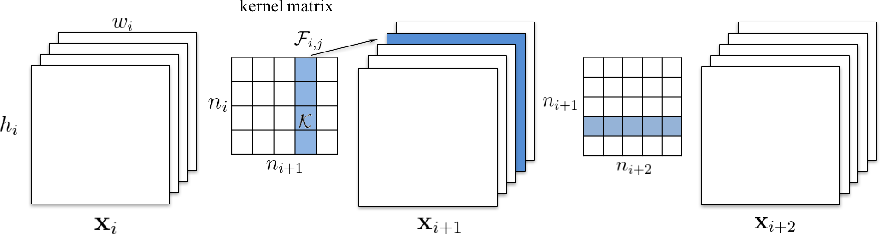
\includegraphics[scale=.75, width=\textwidth]{filter_pruning}
			\caption{ Das Beschneiden eines Filters führt zum Entfernen der entsprechenden Feature-Map und der zugehörigen Kernel in der nächsten Ebene\cite{Filter Pruning}.}
			\label{fig:Filter_pruning}
		\end{figure}
	\item \textbf{Automatische Beschneidung}\\
		Die bisher beschriebenen Kriterien oder die meisten von ihnen fordern, dass das beschnittene Netzwerk noch trainiert wird, um die Endgewichte für die verbleibenden spärlichen Verbindungen zu lernen. Das ganze macht das Pruning-Verfahren noch schwieriger, denn es wird nur dann unterbrochen, wenn der Genauigkeitsverlust wirklich groß ist, was zu viel Zeit in Anspruch nimmt. Um dieses Problem zu lösen, schlagen \emph{Manessi et al}\cite{Automated Pruning}  eine differenzierbare Technik vor, die es ermöglicht, das Pruning durchzuführen, wenn die Gewichte des Netzwerks während der Trainingsphase angepasst werden und die optimalen Schwellwerte automatisch zu suchen. Dieses Verfahren ist inspiriert von dem von Han et al\cite{pruning} und löst viele Probleme, die das Verfahren von \textit{Han et al} nicht lösen könnten oder wegen der Art und Weise, wie sie das Pruning durchführen, entstanden.Erstens werden die Schwellenwerte während des Trainings wie die Gewichte auch gelernt, es kann also eine große Menge von unterschiedlichen Schwellenwerten ausprobiert werden und anstatt der selbe Schwellenwert auf alle Layers anzuwenden, wird jeder Schicht eine Schwelle zugewiesen. Da Nicht alle Layers  gleich empfindlich gegenüber dem Pruning sind und die Verwendung eine selbe Schwelle auf jede Schicht davon ausgeht, dass sie sind, muss dieses Verfahren optimaler.
		Zweitens, anstatt die Trainingszeit zu erhöhen, weil auch neue Parameter gelernt werden müssen, wird sie reduziert,das liegt daran, dass die Netzwerkparameter irgendwann mehr oder weniger spärlich werden, was Feedforward- und Backpropagationzeit erheblich reduziert.Es ist wichtig zu betonen,dass das Netzwerk nur einmal trainiert werden muss, um eine selbe bzw. bessere Genauigkeit wie bzw. als die anderen Methoden zu erzielen.	
\end{itemize}

Aufgrund seiner Automatisierung und Effizienz wird das Pruning in Zukunft sicherlich immer häufiger eingesetzt werden.



\subsection{ Quantisierung von neuronalen Netzwerken}
Im Allgemein wird von Quantisierung gesprochen, wenn es versucht wird, sich den Werten einer großen Menge mit denen einer kleineren Menge zu nähern. Im \ac{ML} ist die Quantisierung der Prozess der Transformation eines ML-Programms in eine approximierte Darstellung mit verfügbaren Operationen mit geringerer Genauigkeit.
\begin{center}
	\textbf{Methoden}
	\begin{itemize}
		\item  Matrixfaktorisierung
		\item Vektorquantisierung
		\item low-bit Quantisierung
	\end{itemize}
\end{center}
\textbf{Matrixfaktorisierung}\\
Die Matrixfaktorisierung versucht, eine Matrix durch die Singulärwertzerlegung($ SVD $) zu approximieren.
Die Singulärwertzerlegung zur Annäherung an eine Matrix $ A \in \R^{m\times n} $ verwendet eine Matrix $ B \in \R^{m\times n}  $ vom Rang $ k \le \min(m, n) $, siehe Gleichung(\ref{eq:SVD}), wobei $ U $ und $ V $ orthogonale Matrizen und $ S $ eine Diagonalmatrix, deren Diagonaleinträge Singulärwerte heißen und bei Betrachtung von oben nach unten monoton abnehmen. Sollte man $ B $ direkt speichern, so hat man keine Kompression gemacht, sondern nur Informationen und Rechenzeiten verschwendet, denn die Matrizen $ A $ und $ B $ haben die gleiche Dimension, also liegt der Hauptvorteil von der Matrixfaktorisierung darin, wie die Matrix $ B $ gespeichert wird.

\begin{equation}\label{eq:SVD}
	\begin{array}{l}
	A = USV^T\\
	B = \widehat{U}\widehat{S}\widehat{V}^T =  U[:,:k] S[:k,:k] V[:k, :]^T \\
	{||A - B||_F} = \sqrt{\sum_{i = 1}^{m} \sum_{j =1}^{n} (A-B)_{i,j}^2} := \text{Frobenius Norm}
	\end{array}	
\end{equation}

Eigentlich werden $ \widehat{U} , \widehat{S} $ und $ \widehat{V} $ statt $ B $ gespeichert, damit wird $ m k + k k + k n $ statt $ mn $ Speicherplatz verwendet und da $ \widehat{S} $ Diagonalmatrix ist, kann auch einfach nur die Diagonaleinträge gespeichert werden, was zu einer Kompressionsrate von $ \dfrac{mn}{k(m+n+1)} $ führt. Die Verwendung von Matrizen von kleinen Rang hebt die Tatsache hervor, dass es redundante Parameter in \ac{NN}-Parametern gibt.Dies Redundanzeigenschaft wird ausgenutzt, um die Geschwindigkeit zu erhöhen\cite[Denton et al]{matrix quantization}.Im Sinne der Frobeniusnorm ist $ B $ die bestmögliche Approximation von $ A $ mit Singulärwertzerlegung durch eine Matrix von Rang $ k $.
Angenommen bildet die zu approximierenden NN-Parameter ein Bild, dann zeigt die Abbildung \ref{fig:matrix_fatorization} ,wie man die NN-Parameter approximieren kann.

\begin{figure}[h]
	\centering
	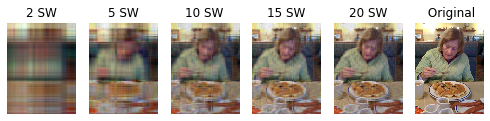
\includegraphics[width=\textwidth]{matrix_fatorization}
	\begin{center}
		SW: Singulärwerte
	\end{center}
	\caption{Parameter Approximieren durch Matrixfaktorisierung }
	\label{fig:matrix_fatorization}
\end{figure}
Wie man in der Abbildung \ref{fig:matrix_fatorization} sieht, reichen  relativ wenige Singulärwerte (ca. $ 5 $) schon aus, um die groben Konturen zu erkennen. Details erkennt man bei ca. $ 10 $ Singulärwerten schon. Generell wird das Bild mit mehr Singulärwerten schärfer.

\textbf{Quantisierung mit weniger Bits(Low-bit Quantization)}\\
Im Bereich des \textit{Deep Learning} ist das Standard numerische Format für Forschung und Einsatz bisher 32-Bit Fließkommazahlen oder FP32, denn es bietet ein bessere Genauigkeit, aber die anderen Formaten wie 8-,4-,2- oder 1-Bits werden auch verwendet, obwohl sie mehr oder weniger ein Verlust an Genauigkeit aufweisen.
Die Verwendung von weniger genauen numerischen Formaten hat nicht nur einen kleinen Verlust der Netzleistung zur Folge, sondern auch die Verwendung von deutlich reduzierter Bandbreite und Speicherplatz. Noch dazu beschleunigt die Quantisierung die Berechnungen, denn die ganzzahlige Berechnung zum Beispiel ist schneller als die Fließkommaberechnung.

Bei Quantisierung mit wenige Bits geht es mehr oder weniger um die Abbildung eine großen Bereiches auf einen kleinen und dazu werden zwei Hauptwerte benötigt: der dynamische Bereich des Tensors und ein Skalierungsfaktor. Angenommen haben wir einen dynamischen Bereich $ [0,500] $ und einen Skalierungsfaktor:$ 5 $, dann ergibt sich der neue Bereich $ [0, 100] $, es wird also Werte zwischen $ [5k, 5(k+1)] $ oder $ [5k -0.5, 5k +0.5] $ auf $ 5k $ abgebildet. Es ist sinnvoller,  die Skalierungsfaktors unter Berücksichtigung der Anzahl und der Verteilung der Werte in dynamischen Bereich des Tensors auszuwählen, sonst können zu viel Informationen verloren gehen.

Sobald ein anderes Format mit weniger Bits als FP32 verwendet, spricht man in \ac{ML} von Quantisierung.
Als Hauptvorteile von Quantisierung haben wir:Erstens wenn wir ein Modell mit FP32-Format durch das gleiche Modell mit 16-Bit Float(FP16), 8-Bit Integer(INT8)  oder 4-Bit Integer(INT4)  ersetzen, reduzieren wir den Speicherbedarf um die Hälfte,um ein Viertel bzw. um ein Achtel.Zweitens sind die Hardwares so programmiert, dass die integer Operationen im Vergleich zu FP32-Operationen schneller und energieeffizienter sind und drittens wird die Bandbreite durch die Verwendung von kleineren Modellen und dynamischen Werten stark reduziert.
		
Zur einer effizienteren Auswahl der Skalierfaktoren pro Schicht bzw. pro Filter ist es notwendig, Statistiken  über das \ac{NN} zu sammeln und das kann \textit{offline} oder \textit{online} gemacht werden. Bei der \textit{Offline} Berechnung werden vor der Bereitstellung des Modells einigen Statistiken gesammelt, entweder während des Trainings oder durch die Ausführung einiger Epochen auf dem trainierten FP32-Modell und basierend auf diesen Statistiken werden die verschiedenen Skalierfaktoren berechnet und nach der Bereitstellung des Modells festgelegt.Bei dieser Methode besteht die Gefahr, dass zur Laufzeit die Werte, die außerhalb des zuvor definierten Bereichs auftreten, abgeschnitten werden, was zu einer Verschlechterung der Genauigkeit führen kann.Bei der \textit{online} werden die \textit{Min/Max}-Werte für jeden Tensor dynamisch zur Laufzeit berechnet. Bei dieser Methode kann es nicht zu einer Beschneidung kommen, jedoch können die zusätzlichen Rechenressourcen, die zur Berechnung der Min/Max-Werte zur Laufzeit benötigt werden, unerschwinglich sein.\cite{quantization1}

Es gibt zwei Quantifizierungsszenarien.Die erste ist das vollständige Training eines Modells mit einer gewünschten niedrigeren Bit-Genauigkeit(\textit{bit precission})(kleiner als 32 Bits).Das Training mit sehr geringer Genauigkeit ermöglicht ein potenziell schnelles Training und Inferenz, aber der Hauptproblem mit diesem Ansatz ist, dass Netzparameter nur bestimmte Werte annehmen können, so ist die Aktualisierung der Netzparameter bzw. das Backpropagation nicht mehr wohldefiniert \cite{quantizationYoni}.
Das zweite Szenario  quantisiert ein trainiertes FP32-Netzwerks mit einer geringeren Bit-Genauigkeit ohne vollständiges Training.Im Allgemeinen gilt: Je geringer die Bitgenauigkeit, desto größer ist der Verlust der Genauigkeit und um diesen Leistungsabfall zu überwinden, wird sehr oft das \ac{NN} erneuert trainiert oder wird auf eine hybride Quantisierung, die zur Quantisierung verschiedene Formaten z.B. INT8 für die Gewichte und FP32 für die Aktivierung gleichzeitig verwendet,  zurückgegriffen.

Vor kurzem haben \cite[Yoni et al]{quantizationYoni} zur  Quantisierung  das lineare Quantisierungsproblem als ein \textit{Minimum Mean Squared Error} (MMSE) Problem formuliert und gelöst.Sie sind in der Lage, die trainierten Modelle zu quantisieren, ohne das \ac{NN} erneuert trainieren zu haben um seine Genauigkeit wiederherzustellen und benutzen dabei nur das INT4-Format. Obwohl diese Methode  minimalen Verlust der Genauigkeit(\textit{accuracy}) aufweist, liefert sie Ergebnisse auf dem neuesten Stand der Technik und nach \cite{quantizationYoni} weist dieser Ansatz den geringeren Genauigkeitsverlust als alle Quantisierungsverfahren auf.

Wie oben erwähnt, eine Quantisierung mit zu weniger Bit führt zu einem großen Genauigkeitsverlust, aber \cite[Yoni et al]{quantizationYoni} haben gezeigt, dass Die Quantisierung mit INT4-Format zu einem besseren Ergebnis führen kann. Das sollte daran liegen, dass sie fürs Approximieren eines Tensors, der gegenüber der Quantisierung sehr empfindlich ist, statt nur einen Tensor mehrere Tensors im INT4-Format benutzen.

\subsection{Huffman Codierung}
Die Huffman-Codierung ermöglicht eine verlustfreie Datenkompression, indem sie jeder einzelnen Dateneinheit  eine unterschiedlich lange Folge von Bits zuordnet.Daraus folgt, dass eine gute Möglichkeit zur besseren Verwaltung der dem Modell zugeordneten Ressourcen ist:Erstmal das Netzwerk zu beschneiden, dann zu quantisieren und am Ende die Huffman-Codierung durchzuführen. 

\section{Experiment} \label{Experiment}

\subsection{Analyse der Ergebnisse mit Hilfe von Metriken}
Nach dem Entwurf des \acsp{NN} muss es noch bewertet werden,um zu überprüfen, ob es unseren Erwartungen (Genauigkeit, Stabilität und Trainingszeit) entspricht. Diese Bewertung kann mit Hilfe von verschiedenen Metriken und einem Testdatensatz gemacht werden.Es ist zwingend erforderlich, dass der Datensatz in zwei (Training und Validierung) oder drei (Training, Validierung und Test) unterteilt wird, da es sonst nicht möglich sein wird, abzuschätzen, wie das Modell Konzepte aus dem Datensatz generalisiert, sondern vielmehr, wie es lernt, jedes Element des Datensatzes einer Klasse zuzuordnen und da das Modell trainiert ist, um die Fehlklassifizierung zu reduzieren, wird die Netzwerkleistung bei Trainingsdaten auf jeden Fall immer besser, daher lohnt es sich nicht zur Abschätzung der Modellleistung die Trainingsdaten zu verwenden.

Metriken werden verwendet, um die Netzwerkleistung zu quantifizieren, und es gibt eine große Vielfalt von ihnen. Die am meistens verwendeten Metriken sind  die mittlere Genauigkeit(\textit{mean accuracy}) und den Logarithmischen Verlust(\textit{logarithmic loss}).

Die Mittlere Genauigkeit oder Klassifizierungsgenauigkeit ist die Anzahl der korrekten Vorhersagen im Verhältnis zu allen getroffenen Vorhersagen. siehe Gleichung(\ref{eq:acc}).
Der logarithmische Verlust sieht genauso wie das \textit{Cross-entropy}(\ref{CE}). Wenn man die Abbildung \ref{fig:accVSlogLoss} genau anschaut, stellt man fest, dass die Genauigkeit nach 60 Epochen flach bleibt, was bedeutet, dass die Netzwerkleistung konstant bleibt, d.h. das Netzwerk keine Verbesserung oder Verschlechterung aufweist.Aber wenn man sich die Validierungsverlustkurve  (\textit{validation loss curve}) betrachtet, stellt man fest, dass die Kurve nach 60 Epochen langsam steigt, was bedeutet, dass die Netzwerkleistung sich verschlechtert.
\begin{equation}\label{eq:acc}
	acc := \dfrac{\textit{Korrekte Vorhersagen}}{\textit{Alle Vorhersagen}}
\end{equation}

\begin{figure}[h]
	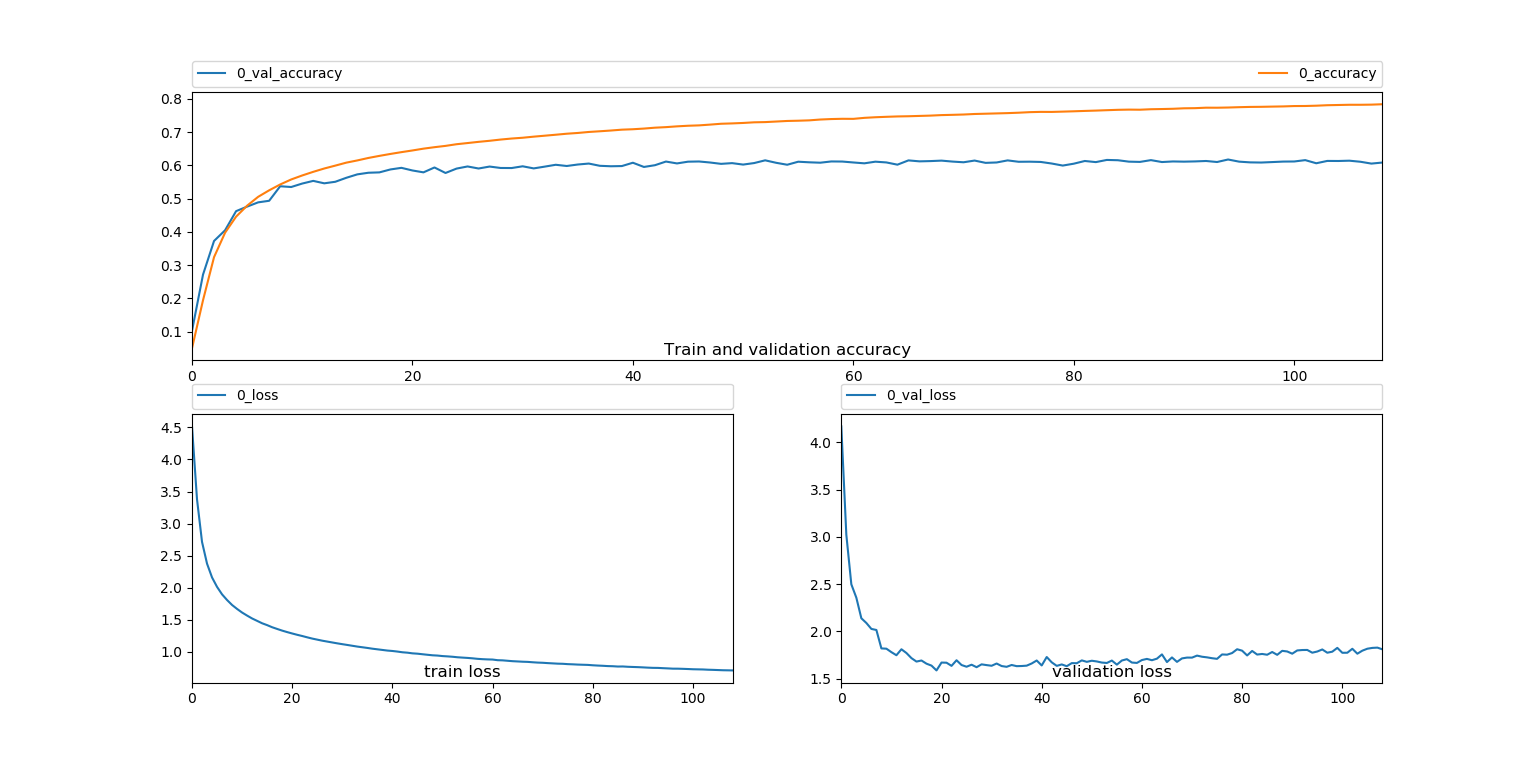
\includegraphics[width=\textwidth]{accVSlogLoss}
	\caption{Vergleich zwischen der Genauigkeitskurve und der logarithmischen Verlustkurve. }
	\label{fig:accVSlogLoss}
\end{figure}

Dieser großer Unterschied liegt daran, dass der logarithmische Verlust die Unsicherheit der Vorhersage in Betracht zieht und die Genauigkeit nicht. Angenommen, das \ac{CNN} klassifiziert eine Klasse $ i $ zweimal hintereinander falsch;$ 0,25 $ und $ 0,012 $ Prozent zum ersten bzw. zweiten Mal; die Netzwerkleistung hat sich verschlechtert, aber die Genauigkeit bleibt gleich, während sich der logarithmische Verlust verschlechtert. \\

 Die Genauigkeit ist keine zuverlässige Metrik für die tatsächliche Leistung eines Klassifikators, da sie bei einem unausgewogenen Datensatz irreführende Ergebnisse liefert (d.h. wenn die Anzahl der Beobachtungen in verschiedenen Klassen stark variiert).
Dies funktioniert nur dann gut, wenn der Datensatz nahezu gleichmäßig auf die Klassen verteilt ist.
\textcolor{purple}{Datenset nicht gleichmäßig verteilen}

\subsection{ Einfluss der Lernrate}\label{Experiment:Lernrate}
Wie in \ref{Lernrate} gesehen, die Lernrate sagt uns, wie schnell wir ans Ziel kommen.
sei $ \eta_{opt} $  bzw. $ \eta $ die optimale bzw. die ausgewählte Lernrate für die Lösung unserer Aufgabe.

 Gilt {$ \eta < \eta_{opt} $}, so sind wir sichern, ein lokales oder globales Minimum zu erreichen.Aber die Anzahl der benötigten Iterationen bis zum Minimum steigt offensichtlich an und das Verfahren kann leichter in einem unerwünschten lokalen Minimum stecken bleiben .
 
 {$ \eta > \eta_{opt} $}:Hier wird die Anzahl der Iterationen entweder reduziert oder erhöht.Das  Verfahren ist im Allgemein nicht stabil, denn es wird über das Minimum ständig hinausgegangen und es ist nicht mehr sichern, zu einem lokalen oder globalen Minimum zu gelangen.  Wenn eine hohe Lernrate angewendet wird, kann man versuchen, das Verhalten des \ac{CNN} zu kontrollieren, indem man die Lernrate nach einer Reihe von Iterationen reduziert, bei denen sich die Metrik (Netzwerkgenauigkeit oder Netzwerkfehler) nicht mehr verbessert hat ,oder indem man Optimierer(\ref{Optimizer}) verwendet, die im Laufe des Trainings die Lernrate entsprechend der Eingabe und der aktuellen Lernrate anpassen. Der Grund, warum die Lernrate immer reduziert und nicht erhöht werden muss, sollte daran liegen, dass das \ac{CNN} irgendwann gut trainiert ist und sollte daher neuen Informationen nicht mehr Gewicht  beimessen als dem bereits Gelernten.


\begin{figure}[h]
	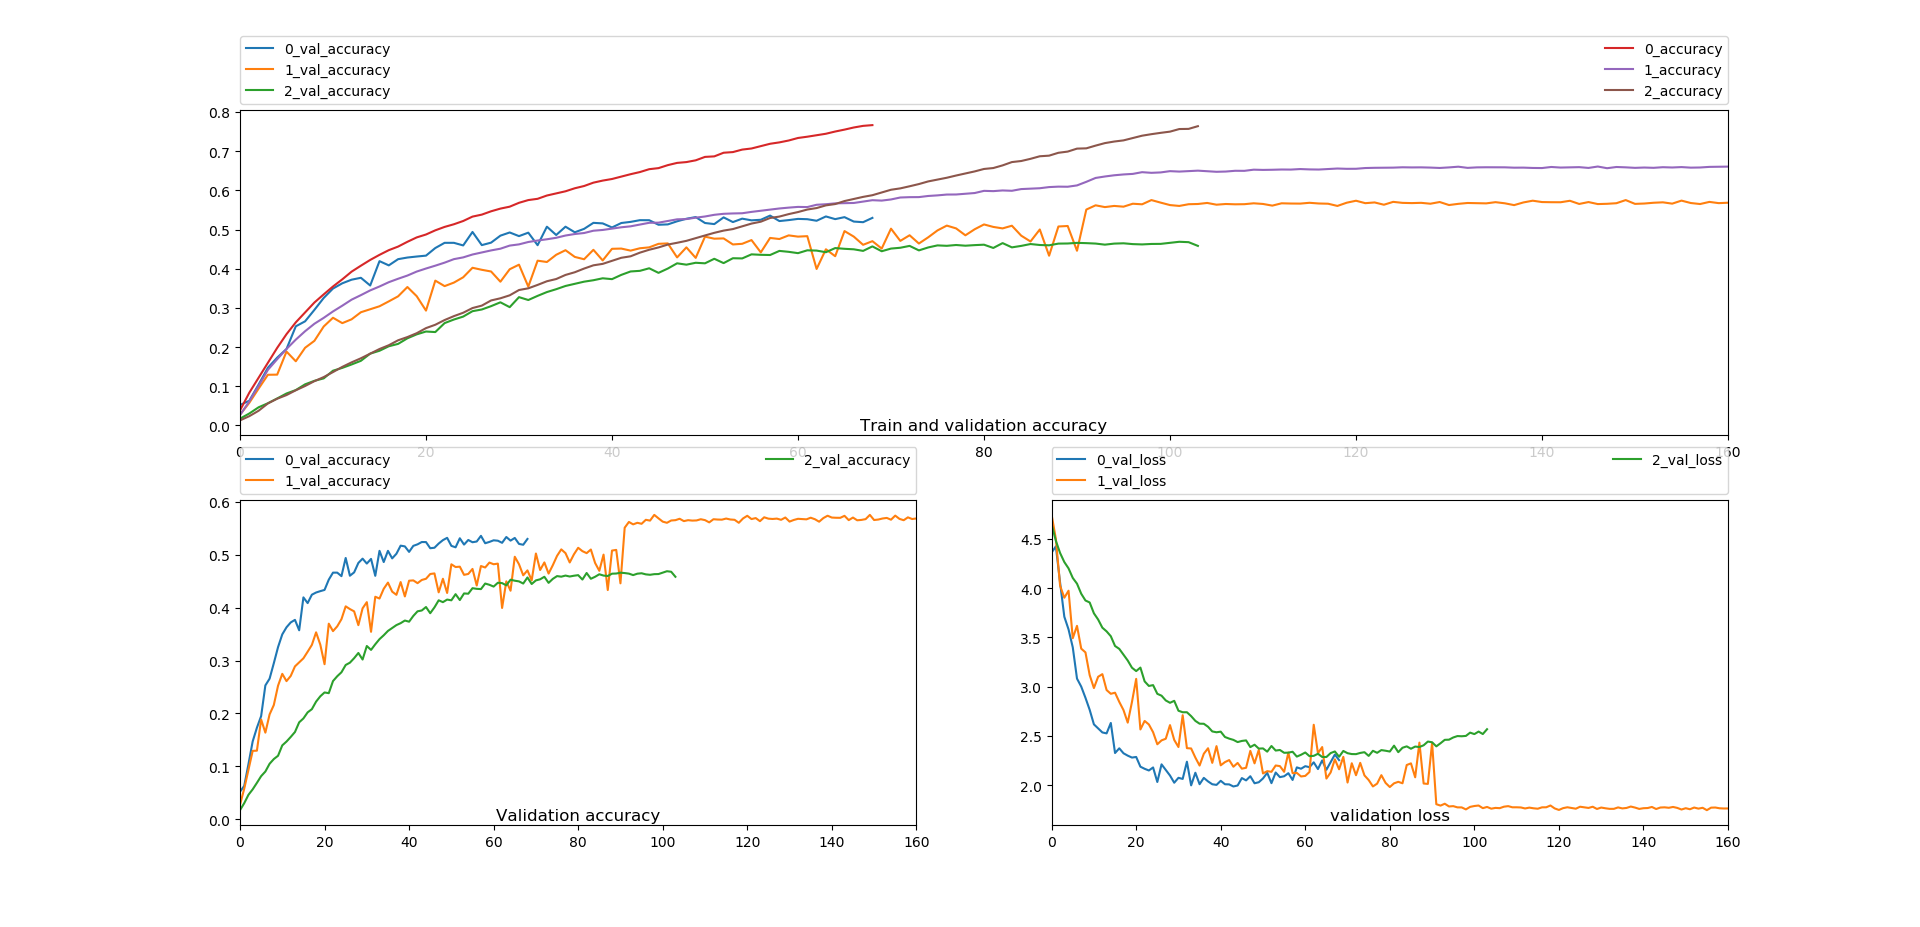
\includegraphics[width=\linewidth]{LearningRate}
	\begin{center}
		\begin{tabular}{r@{: }l r@{: }l}
			Imagegröße & (100, 100,3) & $0\_$ & Lernrate$ =0.0001 $ \\ 
			$ 1\_ $& Lernrate$ =0.005 $ &	$ 2\_ $ & Lernrate$ =0.001 $
		\end{tabular}
		
	\end{center}
\caption{MobileNet\_v1 mit verschiedenen Lernraten.}
\label{fig:Lernrate}
\end{figure}
\begin{itemize}
	\item Aus der Abbildung(\ref{fig:Lernrate}) stellt man zuerst fest, dass die Verwendung verschiedener Lernrate zu unterschiedenen Ergebnissen führt und Je höher die Lernrate, desto mehr Schwankungen gibt es.
	\item Die Reduzierung der Lernrate, wenn sich das Netzwerk nicht mehr verbessert, verbessert die Netzwerkleistung.In der Abbildung gibt es eine jähe Erhöhung der Netzwerkleistung(\textit{orange Kurve}). Das markiert die Änderung der Lernrate von $ 0.005 $ auf $ 0.00001 $. Um zu erkennen, dass sich das Netzwerk nicht mehr verbessert, werden sogenannte \glqq $  Callback$ \grqq-Funktionen verwendet, die fordern, dass bestimmte Hyperparameter wie der Faktor, um den die Lernrate reduziert wird($ new\_lr = old\_lr*factor $) und die Anzahl der Epochen auch \textit{Patience} genannt, die die überwachte Menge(Z.B. der Validierungsfehler oder Validierungsgenauigkeit) ohne Verbesserung produziert haben. Diese Standard-Callback-Funktionen funktionieren leider nur dann gut, wenn der überwachte Menge (pseudo)-monoton(genau wie die ersten beiden Bilder in der Abbildung \ref{fig:Lernrate_scheduler}) ist. Diese Standard-Callback-Funktionen nehmen nicht in Betracht die allgemeine Verhalten des Netzwerks im Zeitintervall \textit{Patience}, sondern vergleichen der erste Eintrag in diesem Zeitintervall mit den anderen Einträgen, was zum Fehler führen kann, wie das letzte Bild in der Abbildung \ref{fig:Lernrate_scheduler} gut zeigt.
	
	Um dieses Problem zu lösen, haben wir eine neue Methode entwickelt, die uns sagt, ob sich die Netzwerkleistung verändert hat und wie sehr sich das Netzwerk verändert hat. Das Verfahren funktioniert wie folgt:
	\begin{itemize}
		\item Wir zeichnen eine horizontale Linie, die über den Durchschnittswert im Zeitintervall \textit{Patience} verläuft.Also $ y = ax +b,( a=0, b= Durchschnittswert) $, siehe orange Kurve in der Abbildung \ref{fig:Lernrate_scheduler}.
		\item Dann versuchen wir alle Werte im Zeitintervall \textit{Patience} durch eine affine Funktion($ y=ax+b $) zu approximieren, indem wir ein \ac{NN} trainieren.Siehe blaue Kurve in der Abbildung \ref{fig:Lernrate_scheduler}.
	\end{itemize}
\end{itemize}

\begin{figure}[h]
	\centering
	\begin{subfigure}{.3\textwidth}
			\centering
			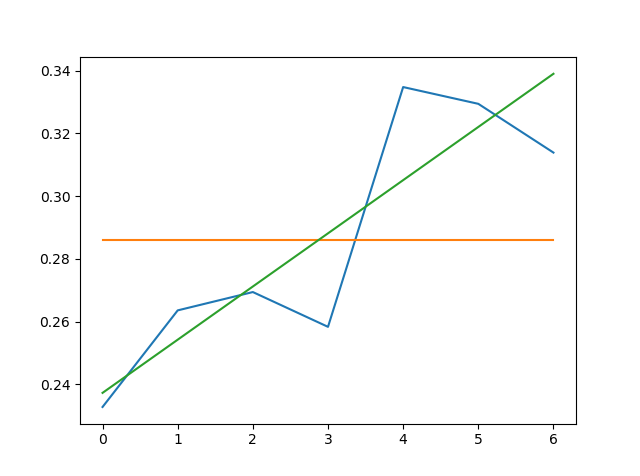
\includegraphics[width=\textwidth]{lr_schedu_Falsch1}
	\end{subfigure}%
	\begin{subfigure}{.3\textwidth}
		\centering
		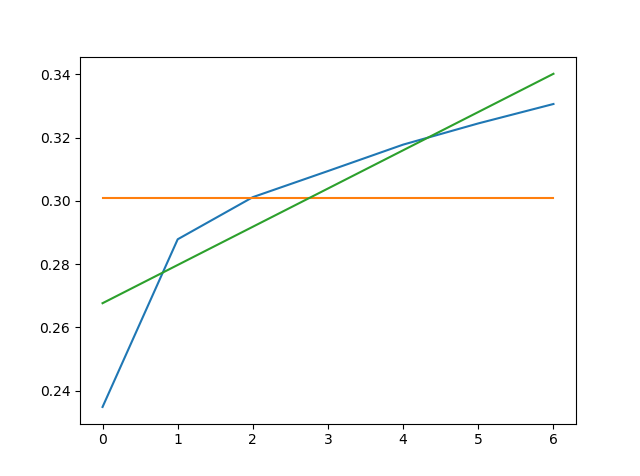
\includegraphics[width=\textwidth]{lr_schedu_Falsch2}
	\end{subfigure}%
	\begin{subfigure}{.3\textwidth}
		\centering
		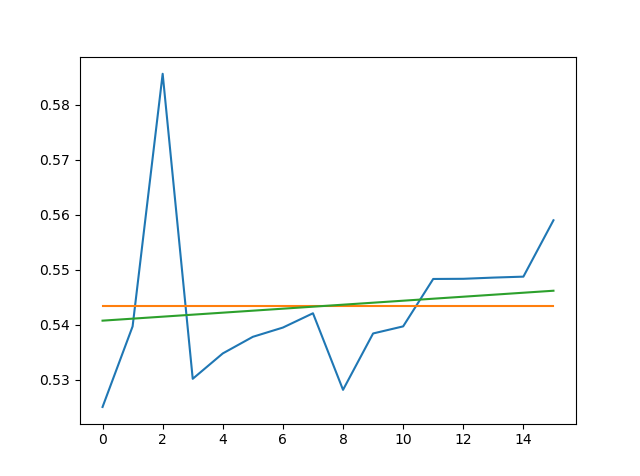
\includegraphics[width=\textwidth]{lr_schedu_Falsch}
	\end{subfigure}
	\caption{Lernraten-Scheduler.}
	\label{fig:Lernrate_scheduler}
\end{figure}

\textcolor{purple}{vergleich zwischen normale LearningRateScheduler und meine}
\subsection{Convolution Layers}
Heutzutage werden am meisten nur Filter der Größe $ 1\times 1 $ und $ 3\times 3 $ und nicht größer verwendet, obwohl größere Filter globale Informationen effizienter entnehmen und so zu besserer Ergebnisse kommen können. Dafür gibt es viele Gründe. Erstens sind die Berechnungen mit kleinerer Filter viel schneller als mit größerer Filter. Zweitens kann ein \ac{ConvL} mit einer großen Filtergröße durch mehrere aufeinanderfolgende \acsp{ConvL} mit einer kleineren Filtergröße ersetzt werden und dabei werden sogar die Anzahl der benötigten Parameter deutlich reduziert. Sollte man z.B. ein $ 5\times 5 $ Filter auf eine Eingabe von Tiefe $ d $ angewendet, so braucht man $ 5\times 5\times d $ Gewichte, um ein Feature-Map zu erzeugen. Nimmt man hingegen zwei aufeinanderfolgende \acsp{ConvL} mit $ 3\times 3$ Filtern, so braucht man nur $ 2(3\times 3\times d) $ Gewichte, um ein Feature-Map zu erzeugen. Drittens hat man bei kleinen Filtern nur eine langsame Reduzierung der Bilddimension, was den Entwurf von sehr tiefer \ac{CNN}s wie \textit{InceptionResNet} ermöglicht. Viertens können kleine Filter sehr lokale Merkmale extrahieren, so dass einfache und komplexe Informationen gleichzeitig erfasst werden.Die Anzahl der extrahierten Features ist enorm und werden gefiltert, wenn man tiefer im Netzwerk geht.

Der Absatz(\ref{ConvL}) behandelte mehr über die Faltungsoperation bei einem Eingang mit einem Kanal. Im Folgenden werden verschiedene Arten beschrieben, wie die Faltungsoperation an einem Eingang mit mehreren Kanälen durchgeführt werden kann. Für die Erklärung von Konzepten wird folgendes als Eingabe der Faltungsschicht betrachtet.

 \[ I=\begin{cases}

 \begin{tabular}{r@{: }l r@{: }l}
 Filtergröße& $ F:=(F_w, F_h) $  & 	$ n_{f}$& Anzahl von Filtern\\
 Input\_{size}& $ W_{in}\times H_{in}\times D_{in} $ & $ P $ & die Anzahl der Nullauffüllung(Padding)
 \end{tabular}
 
 \end{cases}\]


\paragraph{Standard Convolution}

Die Standardfaltung funktioniert genau wie in der Abbildung(\ref{fig:Standardfaltung}).Für eine Eingabe $ I $ erzeugt die Standardfaltung Feature-Maps der Größe $(W_{out},H_{out}, 1) $, wobei $W_{out} $ und $H_{out} $ wie in der Gleichung \ref{eq:outputSize} berechnet werden.Für die Berechnung eines Feature-Map wird ein $ (F_w\times F_h\times D_{in}) $-Filter auf den Input angewendet. Dabei wird zuerst für jeden Kanal $ I_i :=I[:,:, i]$ die Faltungsoperation mit dem Filter $ F_i := F[:,:,i] $ durchgeführt und dann werden die Ergebnisse jeder Faltungsoperation aufsummiert, um das Feature-Map zu bilden.

\begin{equation}\label{eq:outputSize}
	 \begin{split}
	W_{out} &= \frac{W_{in}-F_w+2P}{S}+1\\
	H_{out} &= \frac{H_{in}-F_h+2P}{S}+1\\
	D_{out} &= n_f 
	\end{split} 
\end{equation}
Die Berechnungskosten der Standardfaltung für eine Eingabe $ I $ unter der Annahme, dass die Schrittgröße eins und Padding berechnet werden, entspricht:
\begin{equation}\label{eq:SF_kost}
	F_w\times F_h \times D_{in}\times n_f \times W_{in}\times H_{in}
\end{equation}
\begin{figure}[h]
	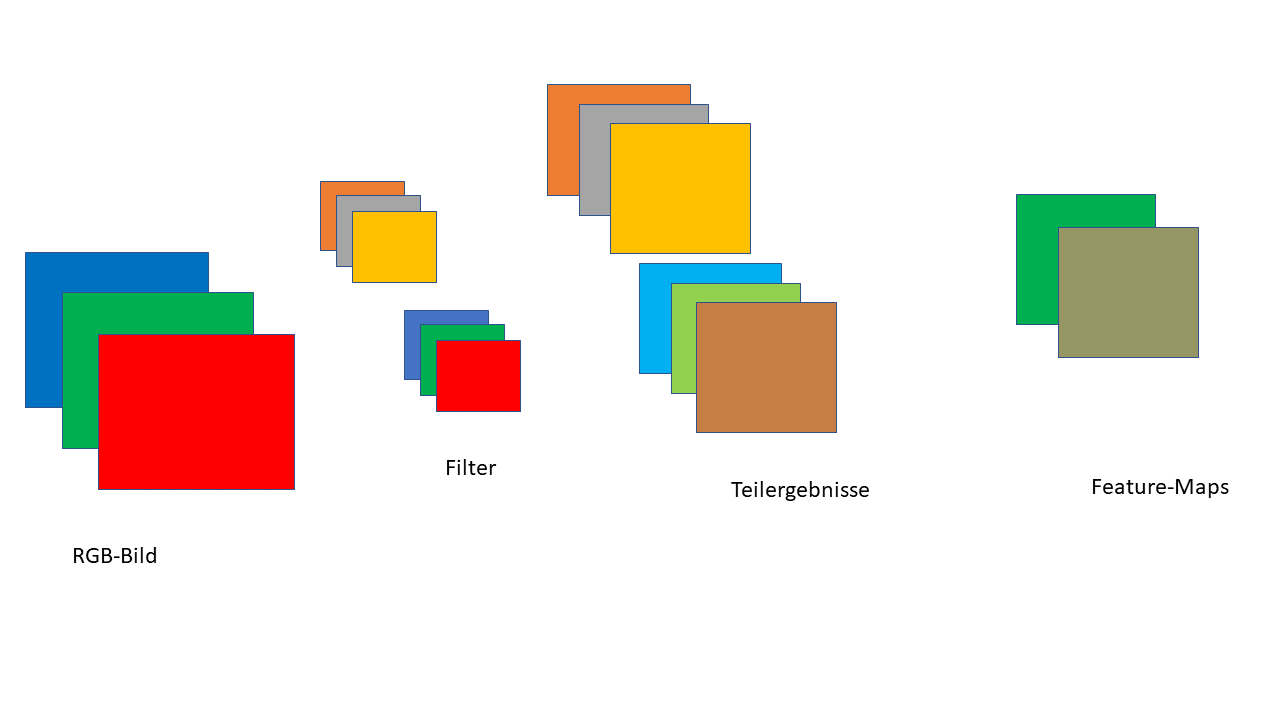
\includegraphics[width=\textwidth]{Convolution/Folie1}
	\caption{Anwendung einer Standardfaltung auf ein Farbbild.}
	\label{fig:Standardfaltung}
\end{figure}

\paragraph{Depthwise Convolution}
Genau wie die Standardfaltung funktioniert die \textit{Depthwise Convolution}, außer dass die Teilergebnisse von Standardfaltung schon der Feature-Maps von der \textit{Depthwise Convolution} entsprechen.Festzustellen ist, dass die Anzahl von Feature-Maps immer proportional zur Anzahl der Kanäle des Inputs sein muss.Damit die Anzahl an Feature-Maps der \textit{Depthwise Convolution} mehr als die Anzahl der Kanäle des Inputs ist, muss ein so genannte \textit{Depth\_multiplier} $ \alpha $ definiert werden. Der \textit{Depth\_multiplier} $\in \N_{\ge1}$ gibt an, wie viele Filter pro Kanal verwendet werden müssen.  Die Abbildung(\ref{fig:Depthwise_faltung}) zeigt die Anwendung der  \textit{Depthwise Convolution} mit einem  $ \alpha=2 $ auf ein Farbbild.
Die \textit{Depthwise Convolution} hat für eine Eingabe $ I $ unter der Annahme, dass Schrittgröße eins und Padding berechnet werden, einen rechnerischen Aufwand von:
\begin{equation}\label{eq:DW_kost}
	F_w\times F_h \times D_{in}\times W_{in}\times H_{in}
\end{equation}
\begin{figure}[h]
	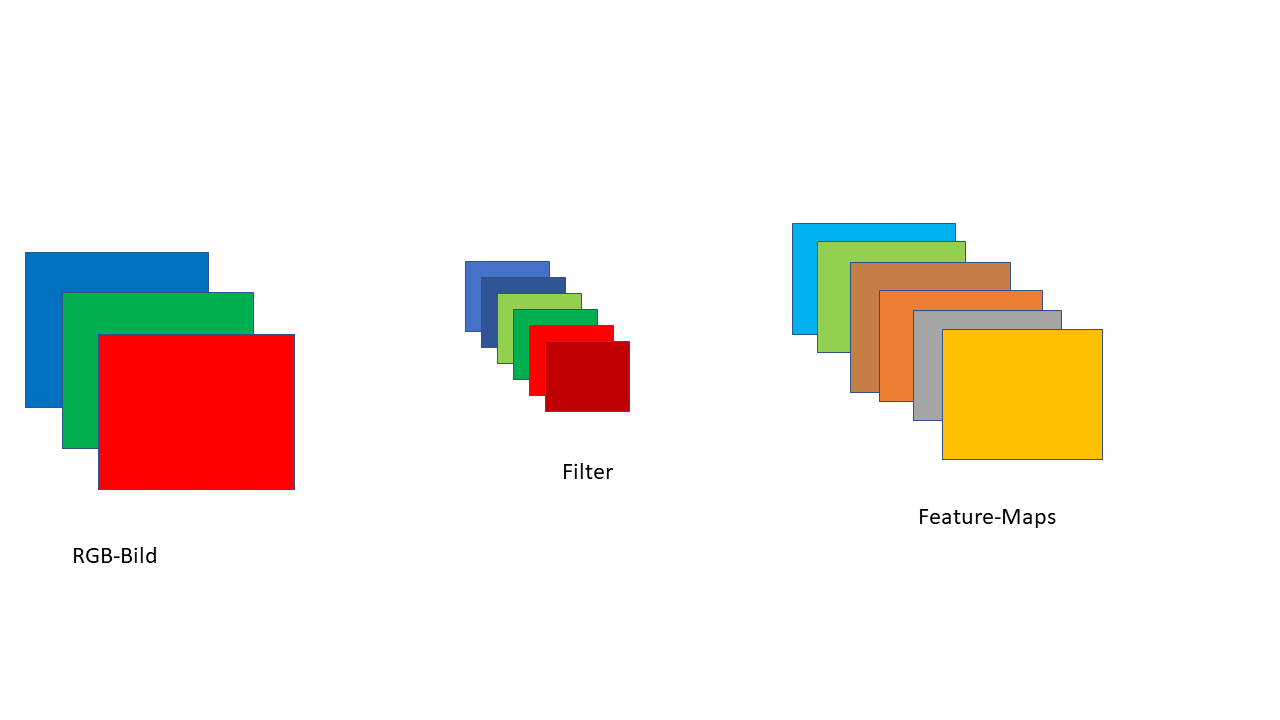
\includegraphics[width=\textwidth]{Convolution/Folie2}
	\caption{Anwendung einer Depthwise Convolution auf ein Farbbild.}
	\label{fig:Depthwise_faltung}
\end{figure}
Wenn man die Gleichungen \ref{eq:SF_kost} und \ref{eq:DW_kost} betrachtet, stellt man schnell fest, dass \textit{Depthwise Convolution} im Vergleich zur Standardfaltung äußerst effizient ist. Der Nachteil von \textit{Depthwise Convolution} ist, dass jede generierte Feature-Map nur einen Kanal in Betracht zieht, was bedeutet, dass Kanäle, die nicht so viele wichtige Informationen enthalten, die gleiche Bedeutung erhalten wie Kanäle, die so viele Informationen enthalten.  

\paragraph{Pointwise Convolution}

Die \textit{Pointwise Convolution} funktioniert genau wie die Standardfaltung, nur dass die Größe der Filter und die Schrittgröße in der Standardfaltung variabel sind und in \textit{Pointwise Convolution} jeweils immer $ (1,1) $ . Also jedes erhaltene Teilergebnis ist nur die Skalierung eines Eingangskanals. Die \textit{Pointwise Convolution} hat für eine Eingabe $ I $ einen rechnerischen Aufwand von:
\begin{equation}\label{eq:PT_kost}
	 D_{in}\times W_{in}\times H_{in} \times n_f
\end{equation}
Die Hauptidee bei der Verwendung der \textit{Pointwise Convolution} ist es, die Korrelation zwischen den Eingangskanälen zu finden, oder lineare Kombinationen zu lernen und erleichtert die Reduzierung und Erhöhung der Anzahl der Kanäle, wenn es zu viele oder zu wenige Feature-Maps gibt. Es kann jedoch mit \textit{pointwise Convolution} kein Feature extrahieren.

\paragraph{Depthwise Separable Convolution} \label{DSC}

Die \textit{Depthwise Separable Convolution}(DSC) besteht aus einer \textit{Depthwise Convolution}, gefolgt von einer \textit{Pointwise Convolution}.Sie kann also Features schneller filtern und kombinieren als die Standardfaltung. Die DSC hat einen rechnerischen Aufwand von:
\begin{equation}\label{eq:DSC_kost}
F_w\times F_h \times D_{in}\times W_{in}\times H_{in} + D_{in}\times W_{in}\times H_{in} \times n_f
\end{equation}

Von \ref{eq:SF_kost} und \ref{eq:DSC_kost} aus sieht man, die DSC weniger Berechnung benötigt als Standardfaltung, und zwar $ \frac{1}{n_f} + \frac{1}{F_w\times F_h}$. Da die DSC zu wenig Parameter verwendet, werden die \ac{CNN}, die die DSC verwenden, als quantisiert bezeichnet.Die DSC ersetzt langsam und sicher die Standardfaltung und das kann man mit $ Xception $ und $ MobileNet $ beobachten.

\textcolor{purple}{compare accuracy von Depthwise Separable Convolution and Standard Convolution}

\subsection{ Vergleich zwischen  Konvolution Neuronale Netzwerke}
\subsubsection{AlexNet}
Wie in \ref{Entwicklung} schon erwähnt, wurde AlexNet von \textit{Krizhevsky} et al \cite{AlexNet} im Jahr 2012 entwickelt. AlexNet hat etwa $ 60 $ Millionen Parametern und etwa $ 650.000 $ Neuronen, besteht aus fünf \acsp{ConvL}, von denen einige von Max-\acsp{PooL} gefolgt sind, und drei \acsp{FCL}(siehe Abbildung \ref{fig:AlexNet}) \cite{AlexNet}. Vor  AlexNet  gab es keine \acsp{CNN} mit so vielen Schichten, noch interessanter sind die Techniken zur Verbesserung der Leistung von  AlexNet :
\begin{itemize}
	\item \textbf{ReLU}: Vor AlexNet waren $ tanh $ und $ sigmoid $ die Standard Aktivierungsfunktionen, aber wegen ihrer Sättigung bei hohen oder sehr niedrigen Werten und der Tatsache, das sie in diesen Bereichen eine Steigung nahe bei null haben, verlangsamen sie stark die Gewichtsanpassungen, was nicht der Fall bei $ ReLU $ ist, das eine Steigung gleich null nur bei negativen Werten und bei positiven höheren Werte  eine Steigung nicht nahe bei null hat. Das Training von \ac{CNN} wird durch $ ReLU $  um ein Vielfaches schneller als ein Äquivalent mit $ tanh $ beschleunigt\cite{AlexNet}.
	
	\item \textbf{Überlappendes Pooling}: Die normalen \acsp{PooL} funktioniert wie in \ref{Pooling Layer} ($ pool\_size = stride$), aber die Überlappenden verwenden einfach ein Schrittgröße kleiner als das $ pool\_size $.Nach \cite{AlexNet} verbessern die überlappenden \ac{PooL}  die Netzgenauigkeit und macht das Netz gegenüber Overfitting robuster.
	\item \textbf{Dropout und Data Augmentation }: Ein anderer Vorteil von AlexNet ist die Verwendung von Dropout(\ref{Dropout}) in \acsp{FCL}, das sich heute als die beste oder eine der besten Regulierungsmethoden erweist, und der Vermehrung der Daten durch Spiegelung, die die Wahrscheinlichkeit von Overfitting und die Anzahl von Epochen reduziert.
\end{itemize}
\begin{figure}[h]
	\centering
	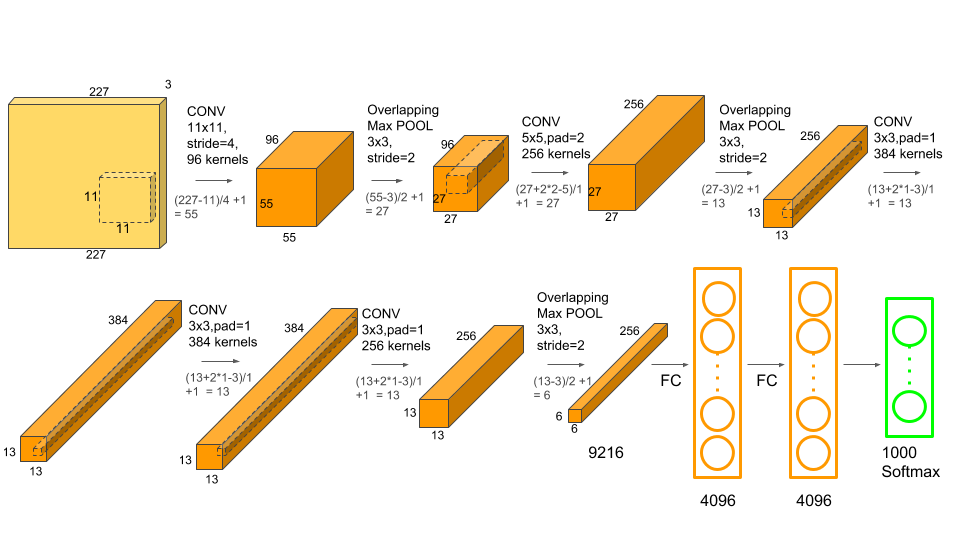
\includegraphics[width=\textwidth ]{AlexNet}
	\caption{ AlexNet Architektur \href{https://neurohive.io/en/popular-networks/alexnet-imagenet-classification-with-deep-convolutional-neural-networks/}{ source} }
	\label{fig:AlexNet}
\end{figure}


AlexNet kann aufgrund seiner Größe($\sim240$MB) nicht immer auf Systemen mit begrenztem Speicherplatz eingesetzt werden, deshalb ist man seit AlexNet ständig auf der Suche nach neuen Architekturen, die weniger Parameter und Speicherplatz brauchen und  gleichzeitig die Ergebnisse auf der Stand der Technik erreichen. Es ist sicherlich  in diesem Zusammenhang, dass viele neue effiziente Modelle wie $ Xception $ und $ MobileNet $ entstanden sind.

\subsubsection{Xception}\label{Xception}
\textit{Xception}(\cite{Xception}) basiert auf  \textit{InceptionV3}(\cite{InceptionV3}). 
Die Inception-Modelle nutzen ein Inception-Block als Baustein. In einem Inception-Block werden mehrere Filter unterschiedlicher Größe separat auf eine Eingabe angewendet und die Ergebnisse jeder Faltungsoperation werden zusammengeführt.Die Verwendung von mehreren Filtern unterschiedlicher Größe ermöglicht eine schnellere Feature-Extraktion, da die kleinen Filter sich mit der Extraktion von sehr lokalen Features beschäftigen, während die großen Filter sich mit der Extraktion von globalen Features beschäftigen. Der Xception-Block (\ref{fig:Xception|MobileNet}) wird mehrmals wiederholt, um das Xception-Modell zu gestalten. Aus der Abbildung \textcolor{purple}{Vergleich Graph  } sieht man an, dass Xception im Vergleich zu anderen Modellen relativ schnell ist.Die Anzahl der Parameter von Xception ist leider immer noch enorm ($ \sim22.000.000 $) .


\begin{figure}[h]
	\centering
	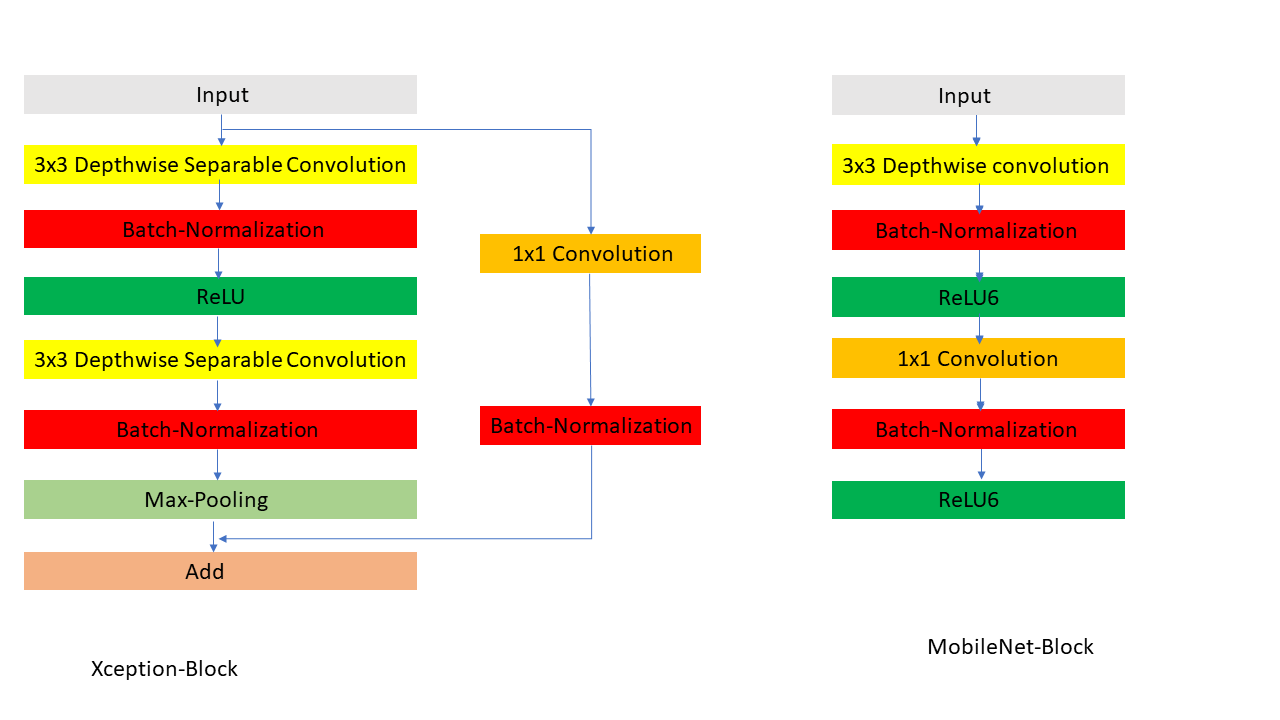
\includegraphics[width=\textwidth ]{Convolution/Folie3}
	\caption{Xception- und MobileNet-Baustein.}
	\label{fig:Xception|MobileNet}
\end{figure}

\subsubsection{MobileNet}
\textit{MobileNet}(\cite{MobileNet}) wie \textit{Xception} macht die \textit{Depthwise Separable Convolution} zunutze.Wie in der Abbildung(\ref{fig:Xception|MobileNet}) zu sehen ist, wurden aber \textit{Batch-Normalisierung und ReLU6}- Layers vor und nach der $ 1\times1 $ Faltungschicht hinzugefügt, was eine schnelle Feature-Extraktion ermöglicht und die \textit{ReLU6} Aktivierung erhöht die Nichtlinearität der Entscheidungsfunktion. \textit{MobileNet} nutzt etwas $\sim 3.500.000$ Parameter, was mindestens sechsmal weniger als die Parameteranzahl von \textit{Xception} ist, was auch eine bessere Inferenz ermöglicht.
\begin{figure}[h]
	\centering
	\includegraphics[width=\textwidth,height=0.8\linewidth]{MobileNet}
	\caption{ MobileNet Architektur }
	\label{fig:MobileNet}
\end{figure}

\subsubsection{TemkiNet}
Inspiriert von den soeben beschriebenen \acsp{CNN} haben wir \textit{TemkiNet} und mehrere Variante davon entwickelt.Die Bausteine von \textit{TemkiNet} sind in der Abbildung \ref{fig:TEMKENG_NET} zu entnehmen
\begin{figure}[h]
	\centering
	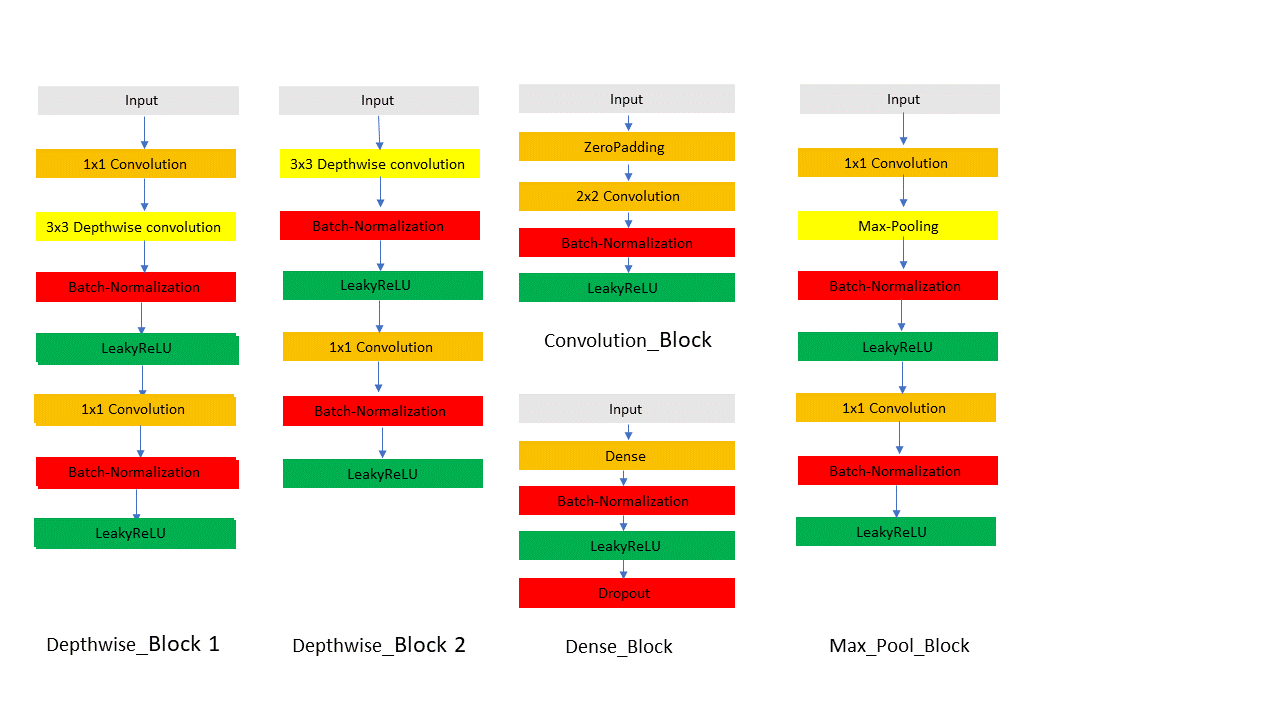
\includegraphics[width=\textwidth ]{Convolution/Folie4}
	\caption{TemkiNet-Bausteine.}
	\label{fig:TEMKENG_NET}
\end{figure}
\begin{table}
	\centering
	\begin{tabular}{|c|c|c|}
		\hline
		Block & Schrittgröße & Outputgröße\\ \hline
		conv\_Block &	$ 2\times2 $ &Bildgröße\\ \hline
		Depthwise\_Block & $ 2\times2 $&Bildgröße/2\\ \hline
		Depthwise\_Block & $ 1\times1 $&Bildgröße/2\\ \hline
		
		Depthwise\_Block & $ 2\times2 $&Bildgröße/4\\ \hline
		$ 2\times $Depthwise\_Block & $ 1\times1 $&Bildgröße/4\\ \hline
		
		Depthwise\_Block & $ 2\times2 $&Bildgröße/8\\ \hline
		$ 3\times $Depthwise\_Block & $ 1\times1 $&Bildgröße/8\\ \hline
		
		Depthwise\_Block & $ 2\times2 $&Bildgröße/16\\ \hline
		$ 4\times $Depthwise\_Block & $ 1\times1 $&Bildgröße/16\\ \hline
		
		Depthwise\_Block & $ 2\times2 $&Bildgröße/32\\ \hline
		$ 2\times $Depthwise\_Block & $ 1\times1 $&Bildgröße/32\\ \hline
		Flatten & / & \\ \hline
		Dense\_Block & / &$ 1024 $\\ \hline
		FC & & $ 101/102 $\\ \hline
		
	\end{tabular}
	\caption{TemkiNet Architektur}
\end{table}
\subsection{Algorithmen zur Optimierung des Gradientenabstiegsverfahren:	Optimizer}\label{Optimizer}
Die Wahl des Optimierungsalgorithmus für ein \ac{CNN} kann den Unterschied zwischen guten Ergebnissen in Minuten, Stunden und Tagen ausmachen.Zum besserer Anwendung der Gradientenabstiegsverfahren wurden mehrere Optimierte Lernverfahren entwickelt. Im folgenden wird ein kurzer Einblick über die bekanntesten Lernverfahren(\textit{Optimizer})  gegeben.\\
Alle heutige Optimizer haben SGD als Vorfahren und der Hauptnachteil von SGD ist , dass es die gleiche Lernrate für die Anpassung aller Netzwerkparameter verwendet und diese Lernrate wird auch während des Trainings nie geändert. 

\subsubsection{Adaptive Gradient Algorithm (AdaGrad)}
AdaGrad bietet während des Netztrainings nicht nur die Möglichkeit, die Lernrate zu verändern, sondern auch für jeden Parameter eine geeignete Lernrate zu finden. Die AdaGrad-Aktualisierungsregel ergibt sich aus der folgenden Formel:
\begin{equation}\label{adagrad}
\begin{aligned}
\alpha_{t}=&\sum_{i = 1}^{t}{(g_{i-1})^2} &
\theta_{t+1} =& \theta_{t} -\eta_{t} g_t \\ \eta_{t} =& \frac{\eta}{\sqrt{\alpha_{t}}+\epsilon}
\end{aligned}
\end{equation}
\begin{center}
	Voreingestellte Parameter(\textit{KERAS}) :
	\begin{tabular}{r@{= }l c@{= }c r@{= }l}
		$ \alpha_{0} $& 0.0 & $ \eta$& 0.001& $ \epsilon $ & $ 10^{-7} $
	\end{tabular}
\end{center}
Dabei wird am Trainingsanfang eine Lernrate für jeden Parameter definiert und im Trainingsverlauf separat angepasst. 
Dieses Verfahren eignet sich gut für spärliche Daten, denn es gibt häufig auftretende Merkmale sehr niedrige Lernraten und seltene Merkmale hohe Lernraten, wobei die Intuition ist, dass jedes Mal, wenn eine seltene Eigenschaft gesehen wird, sollte der Lernende mehr aufpassen. Somit erleichtert die Anpassung das Auffinden und Identifizieren sehr voraussehbarer, aber vergleichsweise seltener Merkmale.\cite{AdaGrad}.Wie in der Gleichung \eqref{adagrad} festzustellen,nach einer bestimmten Anzahl von Iterationen haben wir keine Verbesserung der Netzleistung, denn je größer $ t $ wird, desto kleiner $ \eta_{t} $ wird und irgendwann wird $ \eta_{t} $ so klein, dass $ \eta_{t}g_{t} $ fast gleich null ist.

\subsubsection{Root Mean Square Propagation(RMSProp)}
RMSProp wie AdaGrad findet für jeden Parameter eine geeignete Lernrate und zur Anpassung der Netzparameter basiert der RMSProp Optimizer auf den Durchschnitt der aktuellen Größen der Gradienten statt auf der Summe der ersten Moment wie in AdaGrad.Da $ E[g^2]_t $ nicht schneller als $ \alpha_{t} $\eqref{adagrad} ansteigt, wird die radikal sinkenden Lernraten von Adagrad deutlich verlangsamt.Die Parameteranpassungen richten sich nach der folgenden Gleichung:
\begin{equation}\label{RMSProp}
\begin{split}
E[g^2]_t =\alpha E[g^2]_{t-1} +(1-\alpha)g^2_{t}\\
\theta_{t+1} = \theta_{t} -\frac{\eta}{\sqrt{E[g^2]_t}+\epsilon} g_t, \quad  \epsilon \approx 0
\end{split}
\end{equation}
Der RMSProp funktioniert besser bei Online- und nicht-stationären Problemen.

\subsubsection{Adaptive Moment Estimation(Adam)}
Der Adam\cite{adam} Optimizer ist auch ein adaptiver Algorithmus,der die ersten und zweiten Momente der Gradienten schätzt, um individuelle adaptive Lernraten für verschiedene Parameter zu berechnen.
Adam weist die Hauptvorteile von AdaGrad, das mit spärlichen Gradienten gut funktioniert, und RMSProp, das einige Probleme von AdaGrad löst und das für nicht-konvexe Optimierung geeignet ist,auf.Wie die Parameteranpassung von Adam Optimizer genau funktioniert, ergibt sich aus der folgenden Gleichung: 
\begin{equation}\label{ADAM}
\begin{aligned}
m_{t}=& \beta_{1}m_{t-1}+(1-\beta_{1})g_{t}, &  \widehat{m}_{t} =& \dfrac{m_{t}}{1-\beta_{1}^t}\\
v_{t}=& \beta_{2}v_{t-1}+(1-\beta_{2})g^2_t,&\widehat{v}_{t} =&\dfrac{v_t}{1-\beta_{2}^t}\\
\theta_{t+1} =& \theta_{t} -\dfrac{\eta}{\sqrt{\widehat{v}_{t}}+\epsilon}\widehat{m}_{t}
\end{aligned}
\end{equation}
\begin{center}
	Voreingestellte Parameter(\textit{KERAS}) :
	\begin{tabular}{r@{: }l r@{: }l}
		$ \beta_{1}$ & 0.9 &$ \beta_{2} $& 0.999\\
		$ \eta$& 0.001& $ \epsilon $ & $ 10^{-7} $
	\end{tabular}
\end{center}

Zu weiteren Vorteile der Nutzung von Adam gehört auch seine Einfachheit zur Implementierung, effizienter Nutzung der Speicherplatz und seine Invarianz zur diagonalen Neuskalierung der Gradienten.
\\ \textcolor{purple}{Kleines Experiment}


\subsection{Problem beim Training von  Convolutional   neuronale Netzwerke}
\subsubsection{Overfitting }\label{Overfitting}
%\textcolor{red}{\begin{itemize}
%		\item Erinnern Sie sich an das Kind aus Ihrer Mittelschulklasse, das bei den Tests sehr gut abgeschnitten hat, aber es schlecht tat, wenn die Fragen zum Test ursprüngliches Denken erforderten und nicht in der Klasse behandelt wurden? Warum tat er dies schlecht, wenn er mit einem Problem konfrontiert wurde, das er noch nie zuvor gesehen hatte? Weil er sich die Antworten auf die in der Klasse behandelten Fragen gemerkt hatte, ohne die zugrunde liegenden Konzepte zu verstehen.
%		\item Ebenso ist die Größe des Neuronalen Netzwerks seine Fähigkeit zu lernen, aber wenn Sie nicht vorsichtig sind, wird es versuchen, die Beispiele in den Trainingsdaten zu speichern, ohne das Konzept zu verstehen. Infolgedessen wird das Neuronale Netzwerk außergewöhnlich gut mit den Trainingsdaten arbeiten, aber sie lernen nicht das eigentliche Konzept. Es wird bei neuen und unsichtbaren Testdaten nicht gut funktionieren. Dies wird als Überfitting bezeichnet.
%	\end{itemize}
%}
Wenn ein von der Maschine gelerntes Modell zu gut auf die Trainingsdaten abgestimmt ist und sehr schlechte Vorhersagen über Daten macht, die es bisher nicht gesehen hat, wird gesagt, dass das Modell an Überanpassung(Overfitting) leidet, anders gesagt, das Modell ist nicht in der Lage, die relevanten Merkmale aus den Trainingsdaten zu verallgemeinern, sondern die ganzen Trainingsdaten auswendig zu lernen.Im folgenden werden einige Mittels vorgestellt, um mit Overfitting umzugehen.\\
\begin{center}
	\textbf{Strategie gegen Overfitting}
\end{center}
\subparagraph{{Data Augmentation}}\label{Data Augmentation}
Ein großer Datensatz ist entscheidend für die Leistung tiefer neuronaler Netze.Dass ein Datensatz groß oder ausreichend für das Training eines \ac{CNN}s ist, hängt nur von der Größe des \ac{CNN}s ab und da die \acsp{CNN}, die die besten Leistungen aufweisen, Millionen von Parametern haben, ist für jedes Problem des maschinellen Lernens nahezu unmöglich, ausreichende Daten zu finden.Anstatt immer neue Daten zu sammeln, um die Netzwerkleistung zu verbessern, können wir die Leistung des Modells verbessern, indem wir neue Daten aus bestehenden Daten generieren.\\
Die populären Techniken oder Transformationen zur Vermehrung des Datensatzes sind die horizontalen oder vertikalen Spiegelungen, Drehungen, Skalierungen, Zuschneiden, Parallelverschiebungen und die Gauß'sches Rauschen.
\begin{figure}[h]
	\centering
	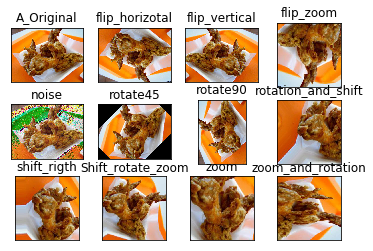
\includegraphics[width=\textwidth]{ImageDataAugmaentation.png}
	\caption{Anwendung von \textit{ImageDataAugmentation} }
	\label{fig:ImageDataAugmentation}
\end{figure}
Für diese Arbeit wurden drei Ansätze zur Erhöhung des Datensatzes verwendet:
Der erste Ansatz besteht darin vor dem Training neue Daten zu erzeugen. Dabei werden die oben erwähnten Techniken vor dem Training angewendet, um zum Trainingszeitpunkt und zur Testzeit einen großen Datensatz zu haben. Der zweite Ansatz verwendet keinen größeren Datensatz, sondern immer das Original. Wenn Samplen aus dem Datensatz in das Netzwerk eingeführt werden, werden sie entweder transformiert oder direkt übertragen.Die \textit{KERAS} Funktion \textit{ImageDataGeneerator} bietet die Möglichkeit, Daten zur Laufzeit umzuwandeln. Vor dem Trainingsanfang werden alle Transformationen, die für jede Sample aus dem Datensatz durchgeführt werden können und beim Einspeisen einer Sample ins Netzwerk wird eine Transformation zufällig auf die Sample durchgeführt. Die Netzwerkeingabe ändern sich also ständig. Das interessanteste an \textit{ImageDataGeneerator} ist, dass es mehrere Transformationen gleichzeitig anwenden(siehe Abbildung \ref{fig:ImageDataAugmentation}). Der dritte Ansatz ist die gleichzeitige Anwendung der beiden anderen Ansätze.\\

\textcolor{red}{In der Abbildung \ref{fig:DataAugmentation} ist zu beobachten, dass die Datenvermehrung die Robustheit des \ac{CNN} erhöht, Trainingszeit erhöht}
Es findet die offensichtlichsten Merkmale, die eine Klasse von einer anderen unterscheiden.
\begin{figure}[h]
	\centering
	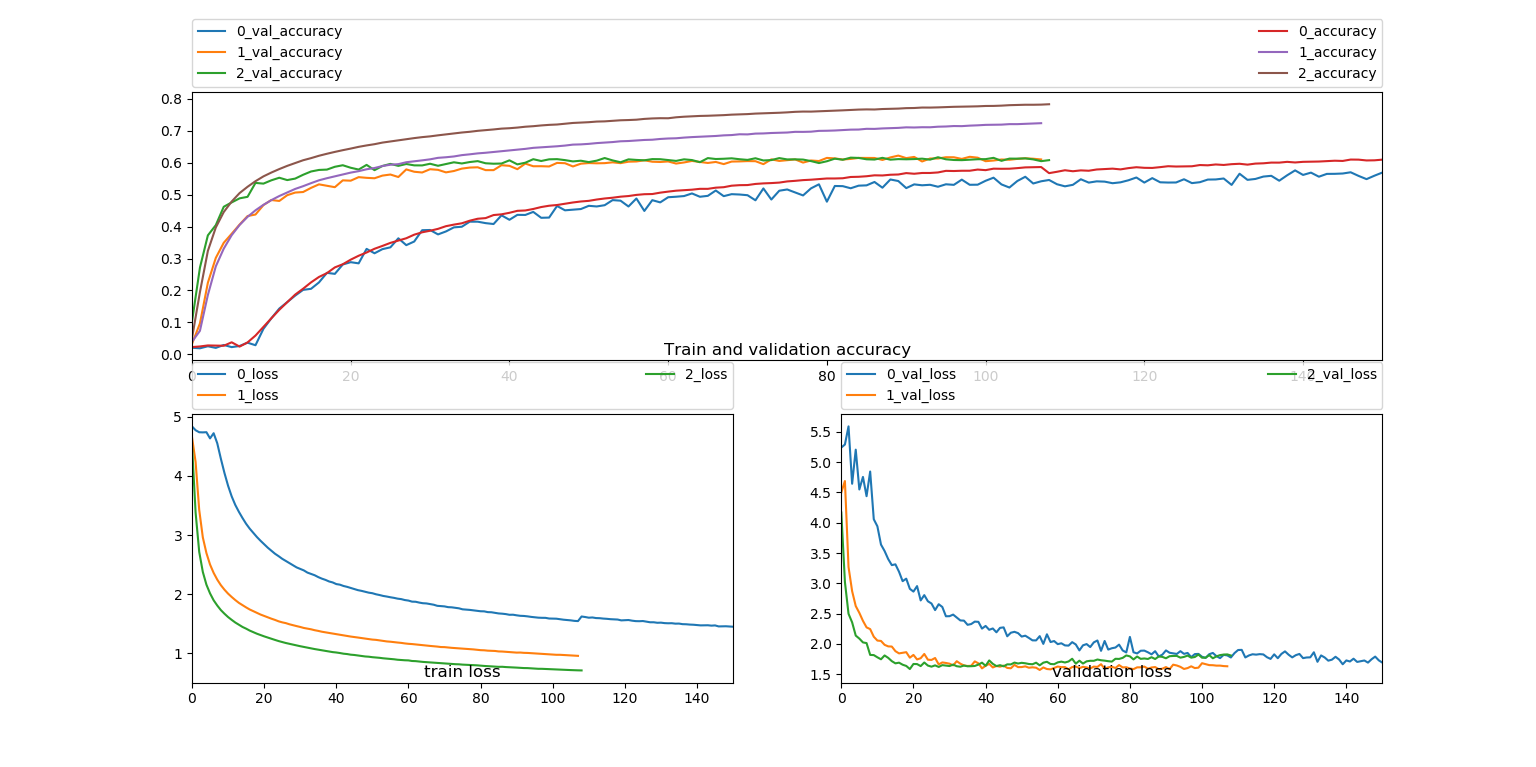
\includegraphics[width=\textwidth]{DataAugmentation.png}
	\caption{Anwendung von \textit{ImageDataAugmentation} }
	\label{fig:DataAugmentation}
\end{figure}


Je mehr Daten verfügbar sind, desto effektiver können die \acsp{CNN} sein. Es ist also mehr als wichtig über eine große Datenmenge zu verfügen. Leider können die gesammelten Datensätze nicht alle mögliche Szenarios des reellen Lebens abdecken,deshalb ist es auch bedeutend, \ac{CNN}  mit zusätzlichen synthetisch modifizierten Daten zu trainieren. Die \acsp{CNN} funktionieren glücklicherweise besser oder immer gut, solange nützliche Daten durch das Modell aus dem ursprünglichen Datensatz extrahiert werden können, selbst wenn die erzeugten Daten von geringerer Qualität sind.\\


\subparagraph{Dropout}  \label{Dropout}
Künstliche Neurone sind von biologischen Neuronen inspiriert, aber die Beiden unterscheidet sich sehr voneinander und einer der wichtigen Unterschiede ist, dass biologische Neuronen unvollkommene Maschinen sind, die sehr oft nicht richtig funktioniert und das ist a priori nie den Fall bei  künstlichen Neuronen. Wir könnten also glauben, dass \ac{KNN} die biologische übertreffen könnten.Es sei denn, dass diese Funktionsstörung von biologischen Neuronen nicht eine Schwäche ist, sondern eher eine Stärke ist.Eine der verblüffenden Entdeckungen in \ac{KI} Bereich ist, dass es wünschenswert ist, künstliche Neuronen von Zeit zu Zeit zu Fehlfunktionen zu bringen\cite{1}. \textcolor{blue}{Jetzt können wir uns fragen, wie Dysfunktion von Neuronen die Performances \acsp{CNN} verbessern kann}.Die zufällige Hinzufügen von Dysfunktionen in einer Schicht der \ac{CNN} wird \textit{Dropout} benannt und wurde von \cite[Geoffrey E. et al]{2} eingeführt.
\subparagraph{Funktionsweise von Dropout}.\\
Genauer gesagt,Dropout bezeichnet die zeitliche zufällige Ausschaltung von Neuronen(versteckt und sichtbar)  in einem  \ac{NN} \cite{3}. Wie die Abbildung \ref{fig:Dropout} zeigt, wenn ein Neuron zufällig aus dem \ac{NN} entfernt wird, werden auch all seine ein- und ausgehenden Verbindungen entfernt.
In einer Dropout-Schicht wird ein Neuron $ \textit{N} $ unabhängig von anderen Neuronen mit einer Wahrscheinlichkeit $ {p} $ zurückgehalten, d.h $ \textit{N} $ wird mit einer Wahrscheinlichkeit von $ {p} $ nicht am Ergebnis der Schicht teilnehmen. Während der Testphase  werden alle Verbindungen zurückgesetzt, die während des Trainings gelöscht wurden und die ausgehenden Verbindungen gelöschter Neurone mit $ p $   multipliziert.

\begin{figure}[h]
	\begin{subfigure}{.5\textwidth}
		\centering
		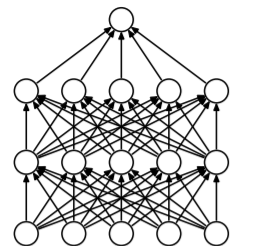
\includegraphics[scale=2, width=.8\linewidth, height=\linewidth]{dropout1.png}
		\caption{Standard neuronale Netze}
		\label{fig:dropout1}
	\end{subfigure}%
	\begin{subfigure}{.5\textwidth}
		\centering
		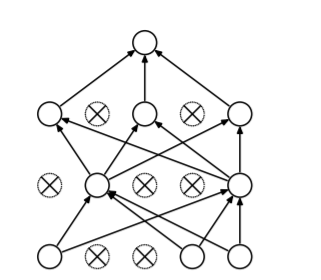
\includegraphics[width=.8\linewidth, height=\linewidth, scale=2]{dropout2.png}
		\caption{Netze nach Dropout}
		\label{fig:dropout2}
	\end{subfigure}
	\caption{Neuronales Netz mit Dropout ausgestattet \cite{3}.}
	\label{fig:Dropout}
\end{figure}

\subparagraph{Verhinderung der Koadaptationen zwischen Neuronen}.\\
Während des Trainings können mehrere Neurone zur Minimierung der Fehlerfunktion so gut zusammenarbeiten, dass die Erkennung bestimmter Merkmale ohne diese Zusammenarbeit nicht mehr möglich ist, aber solche komplexe Koadaptationen  können zu einer Überanpassung führen, denn diese komplexe Koadaptationen existieren nicht immer in Testdaten. Da die am Training teilnehmenden Neuronen nach dem Zufallsprinzip nach jeder Epoche ausgewählt werden, haben wir für jedes Training ein neues Modell, was die Neuronen zur Zusammenarbeit zwingt, ohne jedoch voneinander abhängig zu sein, anders gesagt, wird jedes Neuron unabhängig von anderen Neuronen die Muster korrekt lernen können.  

\subparagraph{Automatische Erhöhung von Training Daten und Regelung }.\\
Noch dazu führt die Ausschaltung von Neuronen, wie es in Abbildung \ref{fig:DropoutDataAugmentation} angezeigt ist, zu einer automatische Erzeugung neuer Trainingsdaten. Die verwendeten Daten in ausgedünnten Modellen sind also nur eine Abstraktion von echten Daten bzw. Rauschdaten und da wir für ein Netz mit $ n $ versteckten Einheiten, von denen jede fallen gelassen werden kann, $ 2^n $ mögliche Modelle haben, haben wir $ 2^n $ mögliche Abstraktion von unseren Daten und das sollte einer der Gründe sein, warum Dropout effektiver als andere rechnerisch kostengünstige Regler ist \cite{3} und warum die Trainingszeit von \acsp{NN} mit Dropout mindestens verdoppelt wird. 

\begin{figure}[h]
	\centering
	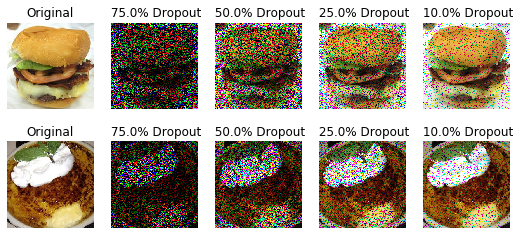
\includegraphics[width=\textwidth]{model}
	\caption{Erhöhung des Trainingsdaten durch Dropout}
	\label{fig:DropoutDataAugmentation}
\end{figure}

Da heutige \acsp{CNN} Million von Neurons haben, wäre es unmöglich alle mögliche ausgedünnte Netzwerke zu trainieren, deshalb ist das Modell, das am Ende des Trainings erhalten wird, nur eine durchschnittliche Approximation aller mögliche Modelle, was schon gut, denn es gibt schlechte und gute Modelle.
%\textcolor{red}{\\\textbf{NICHT LESEN}\\ Wenn ich einem 6-jährigen Aussteiger erklären muss, dann so: Stellen Sie sich ein Szenario vor, in einem Klassenzimmer, ein Lehrer stellt einige Fragen, aber immer die gleichen zwei Kinder beantworten sofort. Nun bittet der Lehrer sie, für einige Zeit still zu bleiben und andere Schüler teilnehmen zu lassen. Auf diese Weise können andere Schüler besser lernen. Vielleicht antworten sie falsch, aber der Lehrer kann sie korrigieren (Gewichtsaktualisierungen). Auf diese Weise lernt die gesamte Klasse (Layer) besser über ein Thema.}

\subparagraph{Batch-Normalisierung}\label{Batch-Normalisierung}
Das Training tiefer neuronaler Netze ist sehr kompliziert und ein Grund dafür ist zum Beispiel die Tatsache, dass die Parameter einer Schicht während des Trainings tiefer neuronaler Netze immer unter der Annahme, dass sich die Parameter anderer Schichten nicht ändern, aktualisiert werden und da alle Schichten während des Updates geändert werden, verfolgt das Optimierungsverfahren ein Minimum, das sich ständig bewegt. Ein anderer Grund dafür ist die ständigen Veränderungen im Laufe des Trainings in die Verteilung des Netzinputs, diese Veränderung wird von \cite{bactchnormalisation} als interne kovariate Verschiebung(\textit{Internal Covariate Shift}) genannt.Zur Lösung dieser Probleme schlagen \textit{LeCunn et al}\cite{LeCun} vor dem Training das Netzinput zu normalisieren. Aber dieser Ansatz bringt nicht so viel, wenn das \ac{NN} wirklich tief ist, denn nur der Netzinput profitiert von der Normalisierung und die kleinen Veränderungen in versteckte Schichten werden sich immer mehr verstärken, je tiefer man das Netz durchläuft. Mit der Ausbreitung tiefer \acsp{NN} dehnt Batch-Normalisierung(BN)\cite{bactchnormalisation} diese Idee der Datennormalisierung auf versteckte Schichten tiefer \acsp{NN} aus. Bei der BN werden die Eingaben in einem Netzwerk standardisiert, die entweder auf die Aktivierungen einer vorherigen Schicht oder auf direkte Eingaben angewendet wird, so standardisiert, dass der Mittelwert in der Nähe von null liegt und die Standardabweichung in der Nähe von eins liegt. Die BN wird über Mini-Batches und nicht über den gesamten Trainingssatz durchgeführt, daher enthalten wir nur Näherungen an tatsächliche Werte der Standardabweichung und des Mittelwerts über das Trainingssatzes, aber wir gewinnen an Geschwindigkeit und an Speicherplatzverbrauch.Die Gleichung \eqref{BNA} gibt die formale Beschreibung des BN Algorithmus an.
\begin{center}
	Batch-Normalisierungstransformation, angewendet auf Aktivierung x über einen Mini-Batch
\end{center}
\begin{subequations}
	\begin{align*}
	\textbf{Input:} & \text{  Werte von x über einer Mini-Batch: } B=\{x_{1...m}\}\\
	& \text{Lernbare Parameter  } \beta, \gamma \\
	\textbf{Output:} & \{ y_i = BN_{\beta, \gamma}(x_i)\}
	\end{align*}
	\begin{align}
	\text{Mini-Batch Mittelwert  : } &\mu_\beta=\frac{1}{m}\sum_{i = 1}^{m}x_i \\
	\text{ Mini-Batch Standardabweichung :} &\sigma_\beta^2=\frac{1}{m}\sum_{i = 1}^{m}(x_i- \mu_\beta)^2 \\
	\text{Normalisierung:} & \widehat{x_i} = \frac{x_i - \mu_\beta}{\sqrt{\sigma_\beta^2 + \epsilon}} \\
	\text{Skalierung und Verschiebung :} & {y_i} = \gamma\widehat{x_i} + \beta \equiv BN_{\gamma, \beta}
	\end{align}
	\label{BNA}
\end{subequations}
Wenn $\gamma = \sqrt{\sigma_\beta^2 + \epsilon}$ und $\beta = \mu_\beta $, bekommen wir die gleiche Verteilung wie vor der Batch-Normalisierung, d.h die Eingabe war also schon normalisiert. Interessanterweise kann das Netz während des Trainings eine bessere Verteilung als die erwünschte finden, denn $\gamma$ und $\beta$ sind lernbare Parameter.

Durch die BN kann zum einen eine hohe Lernrate verwendet,was in tiefer \acsp{NN} ohne BN dazu führen kann, dass die Gradienten explodieren oder verschwinden und in schlechten lokalen Minima stecken bleiben.Die Verwendung einer höhere Lernrate ermöglicht einer schnellere Konvergenz.
Zum anderen wird die interne kovariate Verschiebung geringer, was das Training beschleunigt, in einigen Fällen durch Halbierung der Epochen oder besser. Noch dazu wird das Netz durch die BN in gewissem Maße reguliert, daher wird die Verwendung von Dropout bzw. Regulierungstechnik reduziert oder sogar überflüssig und somit eine Verbesserung der Verallgemeinerungsgenauigkeit.
\subsubsection{Dataset}


\bibliographystyle{acm}
\section{Literatur}
\begin{thebibliography}{lem00}
 \bibitem{1}
	P. Kerlirzin, and F. Vallet: \href{ https://www.mitpressjournals.org/doi/abs/10.1162/neco.1993.5.3.473?journalCode=neco} {Robustness in Multilayer Perceptrons}
	\bibitem{CNNStory}
		Md. Zahangir Alom,Tarek M. Taha, Christopher Yakopcic,Stefan Westberg,Mahmudul Hasan,Brian C. Van Esesn , Abdul A. S. Awwal und Vijayan K. Asari \href{https://arxiv.org/abs/1803.01164}{The History Began from AlexNet: A Comprehensive Survey on Deep Learning Approaches}
	
 \bibitem{2}
 	Geoffrey E. Hinton and Nitish Srivastava and Alex Krizhevsky and Ilya Sutskever and Ruslan R. Salakhutdinov: \href{https://arxiv.org/abs/1207.0580}{Improving neural networks by preventing co-adaptation of feature detectors}
 \bibitem{3}
 	Srivastava, Hinton, Krizhevsky, Sutskever and Salakhutdinov: \href{http://jmlr.org/papers/volume15/srivastava14a.old/srivastava14a.pdf}{Dropout: A Simple Way to Prevent Neural Networks from Overfitting}
\bibitem{4}
Ian Goodfellow, Yoshua Bengio, Aaron Courville:
\href{https://www.amazon.com/Deep-Learning-Adaptive-Computation-Machine/dp/0262035618/ref=as_li_ss_tl?ieTF8&qid=1548018253&sr=8-3&keywords=deep+learning&linkCode=sl1&tag=inspiredalgor-20&linkId=49b3b1cce7e04bb3c9b99f2d878bf805&language=en_US}{Adaptive Computation and Machine Learning series} Page 342
 
 \bibitem{pruning}
	 Song Han, Huizi Mao, William J. Dally \href{https://arxiv.org/abs/1510.00149}{Deep Compression: Compressing Deep Neural Networks with Pruning, Trained Quantization and Huffman Coding}
 \bibitem{Filter Pruning}
 	Hao Li, Asim Kadav, Igor Durdanovic, Hanan Samet, Hans Peter Graf
 	\href{https://arxiv.org/abs/1608.08710}{Pruning Filters for Efficient ConvNets}
 \bibitem{Automated Pruning}
      Franco Manessi, Alessandro Rozza, Simone Bianco, Paolo Napoletano, Raimondo Schettini \href{https://arxiv.org/abs/1712.01721}{Automated Pruning for Deep Neural Network Compression}
      
   \bibitem{matrix quantization}
   		Emily Denton,Wojciech Zaremba,Joan Bruna,Yann LeCun and	Rob Fergus
   		\href{https://arxiv.org/pdf/1404.0736.pdf}{Exploiting Linear Structure Within Convolutional
   			Networks for Efficient Evaluation}
 \bibitem{7}
 	 Pavel Golik , Patrick Doetsch, Hermann Ney
 	\href{http://books.jackon.me/Cross-Entropy-vs-Squared-Error-Training-a-Theoretical-and-Experimental-Comparison.pdf}{Cross-Entropy vs. Squared Error Training:a Theoretical and Experimental Comparison}
 	
 \bibitem{8}
 	\href{http://www.neuronalesnetz.de/aktivitaet.html}{Neuronale Netze:Eine Einführung}
 	
 \bibitem{bactchnormalisation}
	Sergey Ioffe, Christian Szegedy
 	\href{https://arxiv.org/pdf/1502.03167.pdf}{Batch Normalization: Accelerating Deep Network Training b
 		y
 		Reducing Internal Covariate Shift}

	\bibitem{LearningRate}Wikipedia:
		\href{https://en.wikipedia.org/wiki/Learning_rate}{Learning Rate}
	\bibitem{AdaGrad}
		John Duchi,Elad Hazan, Yoram Singer:
		\href{http://www.jmlr.org/papers/volume12/duchi11a/duchi11a.pdf}{Adaptive Subgradient Methods for
			Online Learning and Stochastic Optimization}
	\bibitem{adam}
		Diederik P. Kingma, Jimmy Ba:
		\href{https://arxiv.org/abs/1412.6980}{Adam: A Method for Stochastic Optimization}
		
	\bibitem{quantization1}
		\href{https://nervanasystems.github.io/distiller/quantization.html}{Compressing Models:Quantization}
	\bibitem{quantizationYoni}
		Yoni Choukroun, Eli Kravchik, Fan Yang, Pavel Kisilev:
			\href{https://arxiv.org/abs/1902.06822}{Low-bit Quantization of Neural Networks for Efficient Inference}
	\bibitem{kneuron}
	wikipedia:\href{https://en.wikipedia.org/wiki/Artificial_neuron}{ Artificial neuron}
	\bibitem{AlexNet}Alex Krizhevsky, Ilya Sutskever, Geoffrey E. Hinton
		\href{https://papers.nips.cc/paper/4824-imagenet-classification-with-deep-convolutional-neural-networks.pdf}{ImageNet Classification with Deep Convolutional Neural Networks}
  
  \bibitem{SqueezeNet}
  	Forrest N. Iandola, Song Han, Matthew W. Moskewicz, Khalid Ashraf, William J. Dally, Kurt Keutzer:
  	\href{https://arxiv.org/abs/1602.07360}{SqueezeNet: AlexNet-level accuracy with 50x fewer parameters and <0.5MB model size}
\bibitem{ResNet}
  		Kaiming He, Xiangyu Zhang, Shaoqing Ren, Jian Sun:
  		\href{https://arxiv.org/pdf/1512.03385.pdf}{Deep Residual Learning for Image Recognition}
\bibitem{Xception}
  			François Chollet
  		\href{https://arxiv.org/abs/1610.02357}{Xception: Deep Learning with Depthwise Separable Convolutions}
\bibitem{InceptionV3} Christian Szegedy, Vincent Vanhoucke, Sergey Ioffe, Jonathon Shlens, Zbigniew Wojna
  			\href{https://arxiv.org/abs/1512.00567}{Rethinking the Inception Architecture for Computer Vision}
\bibitem{MobileNet}
			Andrew G. Howard, Menglong Zhu, Bo Chen, Dmitry Kalenichenko, Weijun Wang, Tobias Weyand, Marco Andreetto, Hartwig Adam \href{https://arxiv.org/abs/1704.04861}{MobileNets: Efficient Convolutional Neural Networks for Mobile Vision Applications}
\bibitem{food-101-original}
			Bossard, Lukas and Guillaumin, Matthieu and Van Gool, Luc:\href{https://www.vision.ee.ethz.ch/datasets_extra/food-101/}{Food-101 -- Mining Discriminative Components with Random Forests}
\end{thebibliography}

 
      
  % ggf. hier Tabelle mit Symbolen 
  % (kann auch auf das Inhaltsverzeichnis folgen)

\newpage
  
 \thispagestyle{empty}


\vspace*{8cm}




% Unterschrift (handgeschrieben)



\end{document}
\listoffigures
